\chapter[PhaLP case study: Hyperdimensional protein sequence embedding and binary protein-level classification]{PhaLP case study:\\Hyperdimensional protein sequence embedding\\and binary protein-level classification}
\section{PhaLP database}
To implement and evaluate hyperdimensional computing in typical problem settings in computational biology, the potential of hyperdimensional computing will be evaluated on the PhaLP dataset~\cite{phalp} in this chapter. PhaLP is a comprehensive database currently comprising more than 17,000 entries of phage lytic proteins, including much of their information such as their type, domains and tertiary structures. Phage lytic proteins are used by bacteriophages to infect bacterial cells. To cross the bacterial cell walls, phages use two different types of phage lytic proteins: virion-associated lysins (VALs) and endolysins. Phage lytic proteins also comprise one or more functional domains categorized into two classes: enzymatically active domains (EADs) and cell wall binding domains (CBDs)~\cite{phage}.

The escalating global antibiotic resistance crisis has necessitated the development of alternative strategies to combat bacterial infections~\cite{antibiotic}. One such promising alternative is enzybiotics, a class of enzyme-based antibiotics derived from phage lytic proteins. Phage lytic proteins are produced by bacteriophages during their lytic replication cycle and are responsible for breaking down the bacterial cell wall. As these proteins exhibit a high level of diversity, it is critical to make well-informed selections during the early stages of research and development. In response to this need, Criel \textit{ et al.} introduced PhaLP~\cite{phalp}, a comprehensive, automatically updated, and easily accessible database containing more than 17,000 phage lytic proteins. PhaLP aims to serve as a portal for researchers, allowing them to access all relevant information about the current diversity of phage lytic proteins through user-friendly search engines. This database is specifically designed to facilitate the development and application of enzybiotics by providing a wealth of data on protein architecture, evolution, and bacterial hosts corresponding to the phages. PhaLP not only serves as a valuable starting point for the broad community of enzybiotic researchers but also offers continually improving evolutionary insights that can act as a natural inspiration for protein engineers. By enabling researchers to make well-considered selections of phage lytic proteins during the early stages of their projects, PhaLP plays a significant role in the development of highly effective, narrow-spectrum antibiotics. These enzybiotics have the potential to revolutionize the field of antibacterial agents, offering a much-needed response to the alarming threat of antibiotic resistance that plagues healthcare systems worldwide.

To fully utilize the rich content of PhaLP, the researchers conducted a series of analyses at three levels to gain insights into the host-specific evolution of phage lytic proteins. First, they provided an overview of the modular diversity of these proteins. This was followed by the adoption of data mining and interpretable machine learning approaches to reveal host-specific design rules for domain architectures in endolysins. Lastly, the evolution of phage lytic proteins at the protein sequence level was explored, uncovering host-specific clusters.

In this chapter, we will explore the authors' experiment on protein classification based on sequence data and evaluate the potential of hyperdimensional computing in the context of protein functional annotation. The primary objective is to better understand the role of hyperdimensional computing in protein classification and to elucidate its potential advantages over conventional machine learning techniques.

\section{Type classifcation}
The developers of PhaLP aimed to classify protein sequences based on their type, with a focus on two types of phage lytic proteins: virion-associated lysins (VALs) and endolysins. Both of these proteins play crucial roles in the lytic replication cycle of bacteriophages, as they help the viruses breach the bacterial cell wall. VALs are an integral component of the viral particle, and their primary function is to create a small pore in the peptidoglycan layers of the bacterial cell wall at the infection site. This process allows the bacteriophage to gain access to the interior of the bacterial cell, initiating the lytic replication cycle. On the other hand, endolysins are produced within the infected bacterial cell and act toward the end of the replication cycle. These enzymes degrade the peptidoglycan layer of the bacterial cell wall, leading to cell lysis and the release of new viral particles~\cite{phalp}.

Only a fraction of the database is manually annotated to include the protein's type because the amount of phage lytic proteins whose type is described in the literature is relatively small. The developers of PhaLP resorted to a machine learning approach for the classification of unannotated sequences. The authors embedded each protein sequence \textit{via} SeqVec~\cite{seqvec} and trained a random forest classifier~\cite{randomforest} with 100 estimators and balanced weights to classify the proteins whose types were unknown. For this case study, we attempted to simulate their experiments of classifying the proteins into the two types based on their sequence using several techniques based on hyperdimensional computing.

\section{Methods}
As of March 2023, the latest version of the PhaLP database,~\textit{v2021\_04}, has been used to test our models. This dataset consists of 17,356 unique amino acid sequences of phage-lytic proteins.
\subsection*{Embedding of sequences into hyperdimensional vectors}
First, we used the two sequence encoding techniques as discussed in section~\ref{ssec:protseq} to embed the protein sequences in hyperdimensional space. These methods have been applied to all sequences in the dataset that were manually annotated on their type using both random hyperdimensional vectors and projected ESM-2 embeddings. These were then visually assessed \textit{via} PCA. To confirm the diversity of sequences within the types, pairwise global alignments of every possible non-ambiguous combination of sequences within the two types were performed using the BioAlignments.jl package with a BLOSUM62 scoring matrix and -5 penalty for gaps. All scores within a type are then averaged out.

\subsection*{Classification of hyperdimensional protein sequence embeddings}
To discriminate, we experimented with 3 different methods: the rudimentary hyperdimensional computing classification as seen in section~\ref{sec:example}, an XGBoost classifier and  by A. Hernandez-Cano~\textit{et al.}~\cite{onlinehd}. As in the PhaLP study, we use all non-ML annotated proteins in the dataset. Out of the 11549 unambiguous UniParc accessions in the newest version of the database, 4829 are manually annotated on their type. Out of these manually annotated proteins, 2803 are endolysins and 2026 are VALs. For all classification tests, the F1-score is used as a performance metric as we want to measure the overall performance of the methods. The F1-score is the harmonic mean of the precision and recall and could be interpreted as a weighted accuracy. This accounts for the slight unbalance in the dataset. All methods were evaluated \textit{via} a stratified 10-fold cross validation.
\subsubsection*{Naive additive method}
As a baseline level, we use the rudimentary HDC classification technique as seen in section~\ref{sec:example}: the binary HDVs of sequences of the same class are bundled to construct single HDVs representative of every class. Then, a sequence's class is inferred by comparing the sequence's HDV to both class HDV \textit{via} a similarity measure based on the assumption that the class vector is maximally similar to its components.
\subsubsection*{XGBoost classifier}
The baseline hyperdimensional classification method has been compared to a more established method, the XGBoost classifier~\cite{xgboost}. The classification with an XGBoost classifier is done via the default XGBoost classifier from \textit{XGBoost.jl v2.2.5} using the binary hyperdimensional embeddings as an input.
\subsubsection*{OnlineHD methods}
Another method we experimented with, is OnlineHD by A. Hernandez-Cano~\textit{et al.}~\cite{onlinehd}. It is an algorithm that expands on the classical hyperdimensional training methods by trying to eliminate model saturation. Instead of naively bundling vectors on top of each other, this algorithm assigns weights to every addition depending on how much new information it adds to the model to prevent class vector saturation. To train the model, assume a new data point $V$ with label $l$ and class vectors $C_{i}$ with each having a label $i$. The cosine similarity of $V$ with every class vector is then calculated (denoted as $cos(V, C_{i})$ with $i$ being a label). If $V$ with an actual label $l$ would have been predicted as $l'$, the class vectors will be updated as followed (with learning rate $\eta$ as a tunable hyperparameter):

\begin{alignat}{1}
    \label{eqn:onlinehd}
    C_{l} &\leftarrow C_{l} + \eta (1 - cos(V , C_{l})) * V \\
    C_{l'} &\leftarrow C_{l'} - \eta (1 - cos(V, C_{l'})) * V
\end{alignat}

This means that if a new data point is highly dissimilar to its class vector and thus contains a high amount of new information, the weight of the update ($\eta (1 - cos(V, C_{i}))$) will be high. The information is then also subtracted from the incorrectly predicted class vector. If a label would be correctly predicted for a new data point, the model will not be updated to avoid saturation. To initialize the model, the first vector of a class to be assessed is assumed to be the class vector. For example, if a query vector in our dataset is predicted to be a VAL, but its actual label is endolysin, the class vectors are then updated as followed:

\begin{alignat}{1}
    \label{eqn:onlinehd2}
    C_{VAL} &\leftarrow C_{VAL} + \eta (1 - cos(V, C_{VAL})) * V \\
    C_{endo} &\leftarrow C_{endo} - \eta (1 - cos(V, C_{endo})) * V
\end{alignat}

Due to the nature of this model, we cannot constrict our hyperdimensional embeddings to a bipolar or binary nature anymore and the embeddings are thus allowed to be real-numbered. Mathematical operations such as multiplications and additions are then assumed to be element-wise. On top of the single-pass method as discussed above, A. Hernandez-Cano~\textit{et al.} also implemented an iterative retraining algorithm to increase the accuracy of OnlineHD. This starts from the class vectors made \textit{via} the single-pass OnlineHD model, but assesses the class vectors by performing inference with every training vector. If a training vector's label is wrongly predicted, equations 4.1 and 4.2 are then used to update the model. This entire sequence is iterated over a given amount of cycles.

Since these algorithms are only available as PyTorch implementations, implementations in Julia have been made here. A stratified 10-fold cross validation of these models with our subject sequences has been performed. The learning rate is set at 0.035 for both the single-pass and the iterative method and the amount of retraining iterations for the iterative method is set to 120 as these are the values set by default in their PyTorch package. To test these algorithms, real-numbered embeddings had to be made from our subject sequences. So instead of embedding the sequences starting with random bitvectors, random vectors with values in interval $[-1, 1]$ for both the random amino acid vectors and projected ESM-2 embeddings were made to obtain real-valued hyperdimensional vectors for every amino acid. The same bag-of-words and convolutional approaches as discussed in Section~\ref{ssec:protseq} have been applied here to obtain real-valued sequence embeddings. These were assessed \textit{via} a scatter-plot of the two first principal components of their PCA projection.

To monitor the training procedure of an OnlineHD single-pass model, the same procedures as above are followed, but without the cross validation. The absolute difference between the cosine similarities, $cos(V, C_{VAL})$ and $cos(V, C_{VAL})$ as described in equations 4.3 and 4.4, has then been calculated for each query vector before the update. The results are shown in Figure~\ref{fig:main2} for every combination of amino acid- and sequence embedding methods. Another approach to monitor the training procedure is to track the two class vectors $C_{VAL}$ and $C_{endo}$ individually. For each query vector $V_{l}$ with a known label $l$, we calculate the cosine similarity $cos(V_{l}, C_{l})$. The results are shown in Figure~\ref{fig:main} for every combination of amino acid- and sequence embedding methods. 

To follow the training procedure in terms of performance, the dataset is divided into training and testing sets, while ensuring stratification is preserved, with the test set comprising 10 \% of the data. The training data is further partitioned into 500 batches, and the model is trained incrementally using these batches. After each batch has been processed, the model's performance on the test data is assessed to provide insights into its learning trajectory with the results shown in Figure~\ref{fig:main39} for every combination of amino acid- and sequence embedding methods.

\section{Results}
\subsection*{Embedding of sequences into hyperdimensional vectors}
There is no visual difference between the PCA plots for the sequences embedded \textit{via} the bag-of-words method and the convolutional method, but there is a clear difference between the different starting embeddings as seen in Figure~\ref{fig:phalp_emb}. The binary sequence embeddings from both the bag-of-words method and the convolutional method made with ESM-2 AA embeddings seem to capture more of the variance between the sequences.

\begin{figure}[ht!]
    \centering
    \begin{subfigure}{0.48\textwidth}
        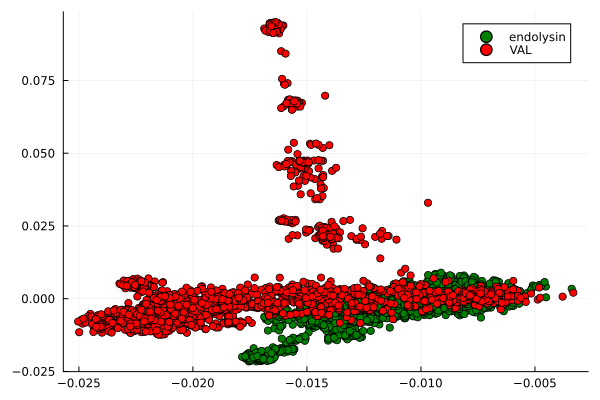
\includegraphics[width=\textwidth]{phalp_bow_rand}
        \caption{BoW-encoded protein sequences, starting from random vectors. These PCs account for roughly 7 \% of the total variance in the system.}
    \label{fig:phalpbowrand}
    \end{subfigure}
    \hfill
    \begin{subfigure}{0.48\textwidth}
        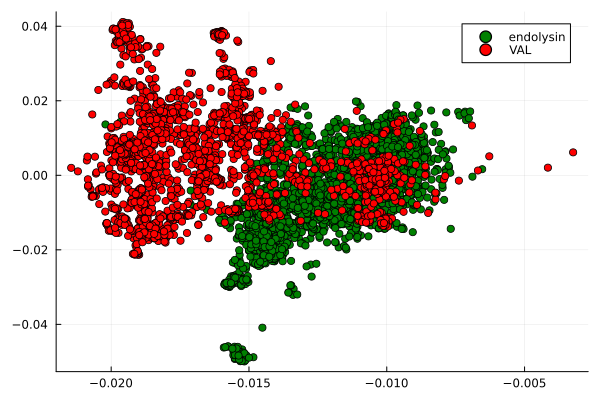
\includegraphics[width=\textwidth]{phalp_bow_esm}
        \caption{BoW-encoded protein sequences, starting from projected ESM-2 embeddings. These PCs account for roughly 15.5 \% of the total variance in the system.}
    \label{fig:phalpbowesm}
    \end{subfigure}
    
    \begin{subfigure}{0.48\textwidth}
        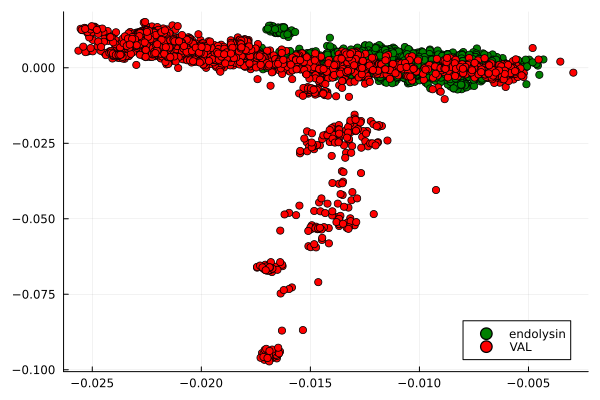
\includegraphics[width=\textwidth]{phalp_cnn_rand}
        \caption{Convolutionally encoded protein sequences, starting from random vectors. These PCs account for roughly 7 \% of the total variance in the system.}
    \label{fig:phalpcnnrand}
    \end{subfigure}
    \hfill
    \begin{subfigure}{0.48\textwidth}
        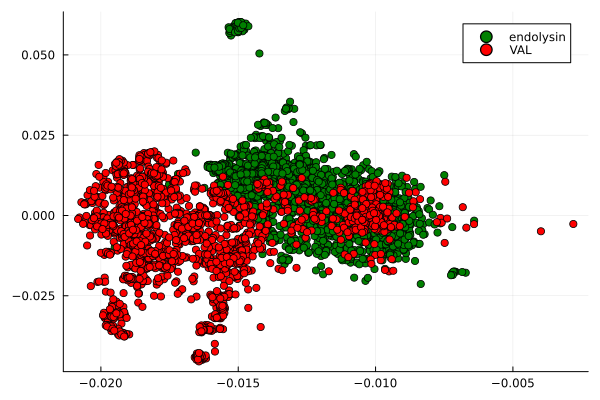
\includegraphics[width=\textwidth]{phalp_cnn_esm}
        \caption{Convolutionally encoded protein sequences, starting from random vectors. These PCs account for roughly 15.5 \% of the total variance in the system.}
    \label{fig:phalpcnnesm}
    \end{subfigure}
    \caption{Scatter-plot of the first two principal components of the binary encoded phage lytic proteins \textit{via} the BoW-method starting from (a) random HDVs per amino acid (b) projected ESM-2 amino acid embeddings and \textit{via} the convolutional method from (c) random HDVs per amino acid (d) projected ESM-2 amino acid embeddings. Only manually annotated phage lytic proteins were considered and are color-coded based on their type.}
    \label{fig:phalp_emb}
\end{figure}

As with the binary embeddings, PCA of the real-valued sequence embeddings shows no distinction between those made \textit{via} the bag-of-words method and the convolutional method whilst showing a clear difference between the different starting embeddings as seen in Figure 4.3. Similarly, the explained variance is much higher for embeddings made with projected ESM-2 embeddings. However, the PCA method retrieves much more information from real-valued embeddings. From all the PCA scatter plots mentioned, we can estimate by the sparser distribution of the VAL proteins that these would be slightly more diverse in sequence than endolysins.

\begin{figure}[ht!]
    \centering
    \begin{subfigure}[b]{0.48\textwidth}
        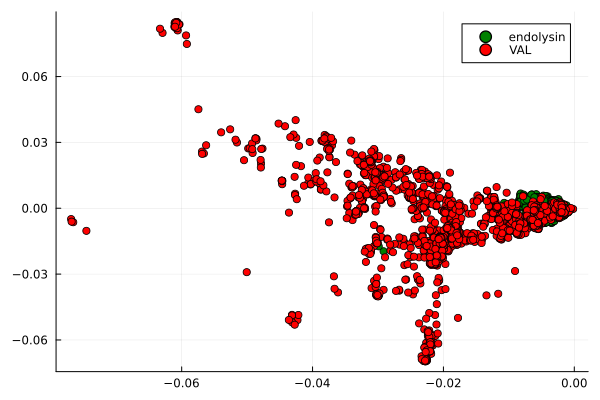
\includegraphics[width=\textwidth]{phalp_bow_rand_real}
        \caption{BoW-encoded protein sequences, starting from random vectors. These PCs account for roughly 30.4 \% of the total variance in the system.}
    \label{fig:phalpbowrandr}
    \end{subfigure}
        \hfill
    \begin{subfigure}[b]{0.48\textwidth}
        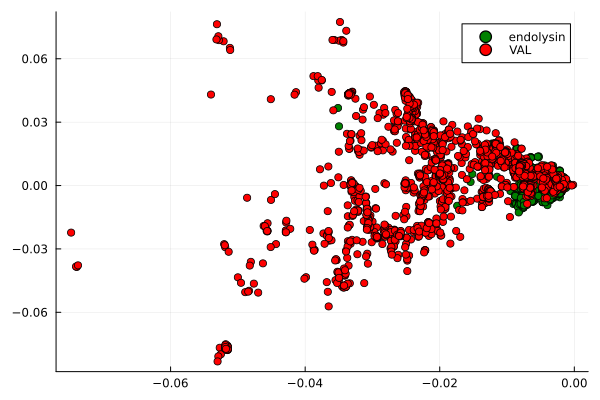
\includegraphics[width=\textwidth]{phalp_bow_esm_real}
        \caption{BoW-encoded protein sequences, starting from projected ESM-2 embeddings. These PCs account for roughly 57.3 \% of the total variance in the system.}
    \label{fig:phalpbowesmr}
    \end{subfigure}
    \begin{subfigure}[b]{0.48\textwidth}
        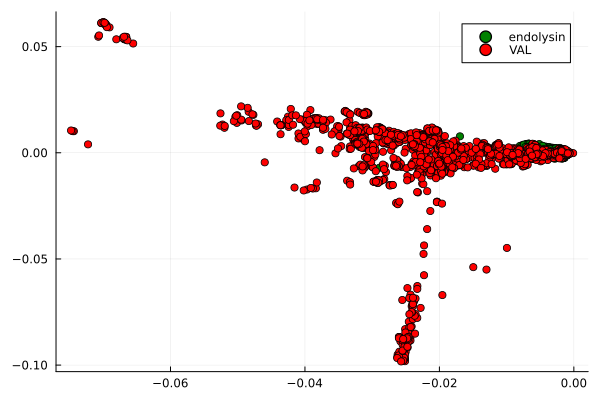
\includegraphics[width=\textwidth]{phalp_rand_esm_real}
        \caption{Convolutionally encoded protein sequences, starting from random vectors. These PCs account for roughly 30.4 \% of the total variance in the system.}
    \label{fig:phalpcnnrandr}
    \end{subfigure}
    \hfill
    \begin{subfigure}[b]{0.48\textwidth}
        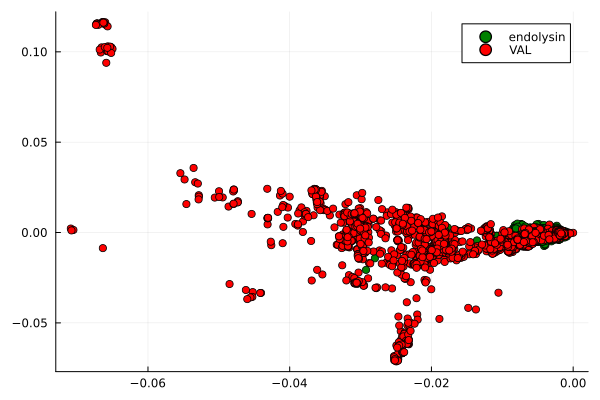
\includegraphics[width=\textwidth]{phalp_cnn_esm_real}
        \caption{Convolutionally encoded protein sequences, starting from projected ESM-2 embeddings. These PCs account for roughly 57.3 \% of the total variance in the system.}
    \label{fig:phalpcnnesmr}
    \end{subfigure}
    \caption{Scatter-plot of the first two principal components of the real-valued encoded phage lytic proteins \textit{via} the BoW-method starting from (a) random HDVs per amino acid (b) projected ESM-2 amino embeddings and \textit{via} the convolutional method from (c) random HDVs per amino acid (d) projected ESM-2 amino embeddings. Only manually annotated phage lytic proteins were considered and are color-coded based on their type.}\label{fig:phalp_embr}
\end{figure}

In each of the PCA projections previously discussed, VALs consistently exhibited a higher degree of diversity in comparison to endolysins. To validate this observation, pairwise alignments were conducted across all sequences within their respective groups. VAL proteins yielded an average score of -209, while the endolysins scored -7. This pronounced disparity in scores shows greater intra-group dissimilarity among the VAL sequences as opposed to those of the endolysins, confirming our findings in the PCA projections.

\subsection*{Classification of hyperdimensional protein sequence embeddings}
The resulting F1-scores from our 4 classification methods are listed in Table~\ref{tab:phalpclass}. Evaluating our naive additive model using stratified 10-fold cross-validation results in F1-scores of around 0.14 for every kind of amino acid embedding.

\begin{table}[h]
    \caption{\label{tab:phalpclass}Results of type classifications using the principal classification technique of hyperdimensional computing, an XGBoost classifier and OnlineHD implementations with several kinds of embeddings. Note that the OnlineHD-based models were developed using real-valued embeddings.}
    \resizebox{\textwidth}{!}{\begin{tabular}{ccccc}
        \hline
        \underline{F1-scores} & \textbf{BoW/random} & \textbf{BoW/ESM} & \textbf{Convolutional/random} & \textbf{Convolutional/ESM} \\
        \hline
        \textbf{Naive addition} & 0.1458 & 0.1468 & 0.1461 & 0.1461 \\
        \hline
        \textbf{XGBoost classifier} & 0.9667 & 0.9754 & 0.9661 & 0.986 \\
        \hline
        \textbf{Single-pass OnlineHD} & 0.8901 & 0.9214 & 0.7793 & 0.8400 \\
        \hline
        \textbf{Iterative OnlineHD} & 0.9487 & 0.9757 & 0.9486 & 0.9670 \\
        \hline
    \end{tabular}}
\end{table}

The scores of the XGBoost classifier with our sequence embeddings are much more comparable to the results of the experiment in the PhaLP paper, with the convolutional embeddings generally performing better than the bag-of-words embeddings and also the ESM 2-based performing better than random base vectors when considering the type of amino acid vectors used. This is an indication that hyperdimensional computing can provide a very fast and reliable method of embedding protein sequences, even without prior biological information. The drawback of this machine learning model, which is to be expected from every gradient-based model, is that training and predictions take much longer to compute compared to hyperdimensional training models. The cross validation procedure took up to 5 minutes on a consumer-grade laptop, whilst with the naive additive approach, the procedure took less than 10 seconds to finish.

Comparing the results of the OnlineHD models to the naive additive HDC model, we can see a substantial increase in the performance of this model. The single-pass model seems to have more widely varying results depending on the type of embeddings used. As opposed to the XGBoost classifier, it performs better using bag-of-words embeddings. The model also performs better when trained with embeddings based on projected ESM-2 vectors. Iterative retraining of the model seems to increase its performance significantly, even coming close to the performance of an XGBoost classifier in this case. Further improvement might be found when optimizing the models' parameters. The cross validation procedure takes less than 10 seconds to run for the single-pass model, whilst doing an iterative retraining of the model adds 2 to 3 minutes. This model appears to be a decently performing extension of the rudimentary hyperdimensional classification model for protein classification, whilst still being much more efficient than the commonly used machine learning models. The drawback of the model is that we cannot use hyperefficient bit-operations anymore, which limits its efficiency compared to the binary nature of the additive model.

\begin{figure}[ht!]
    \centering
    \begin{subfigure}{0.48\textwidth}
        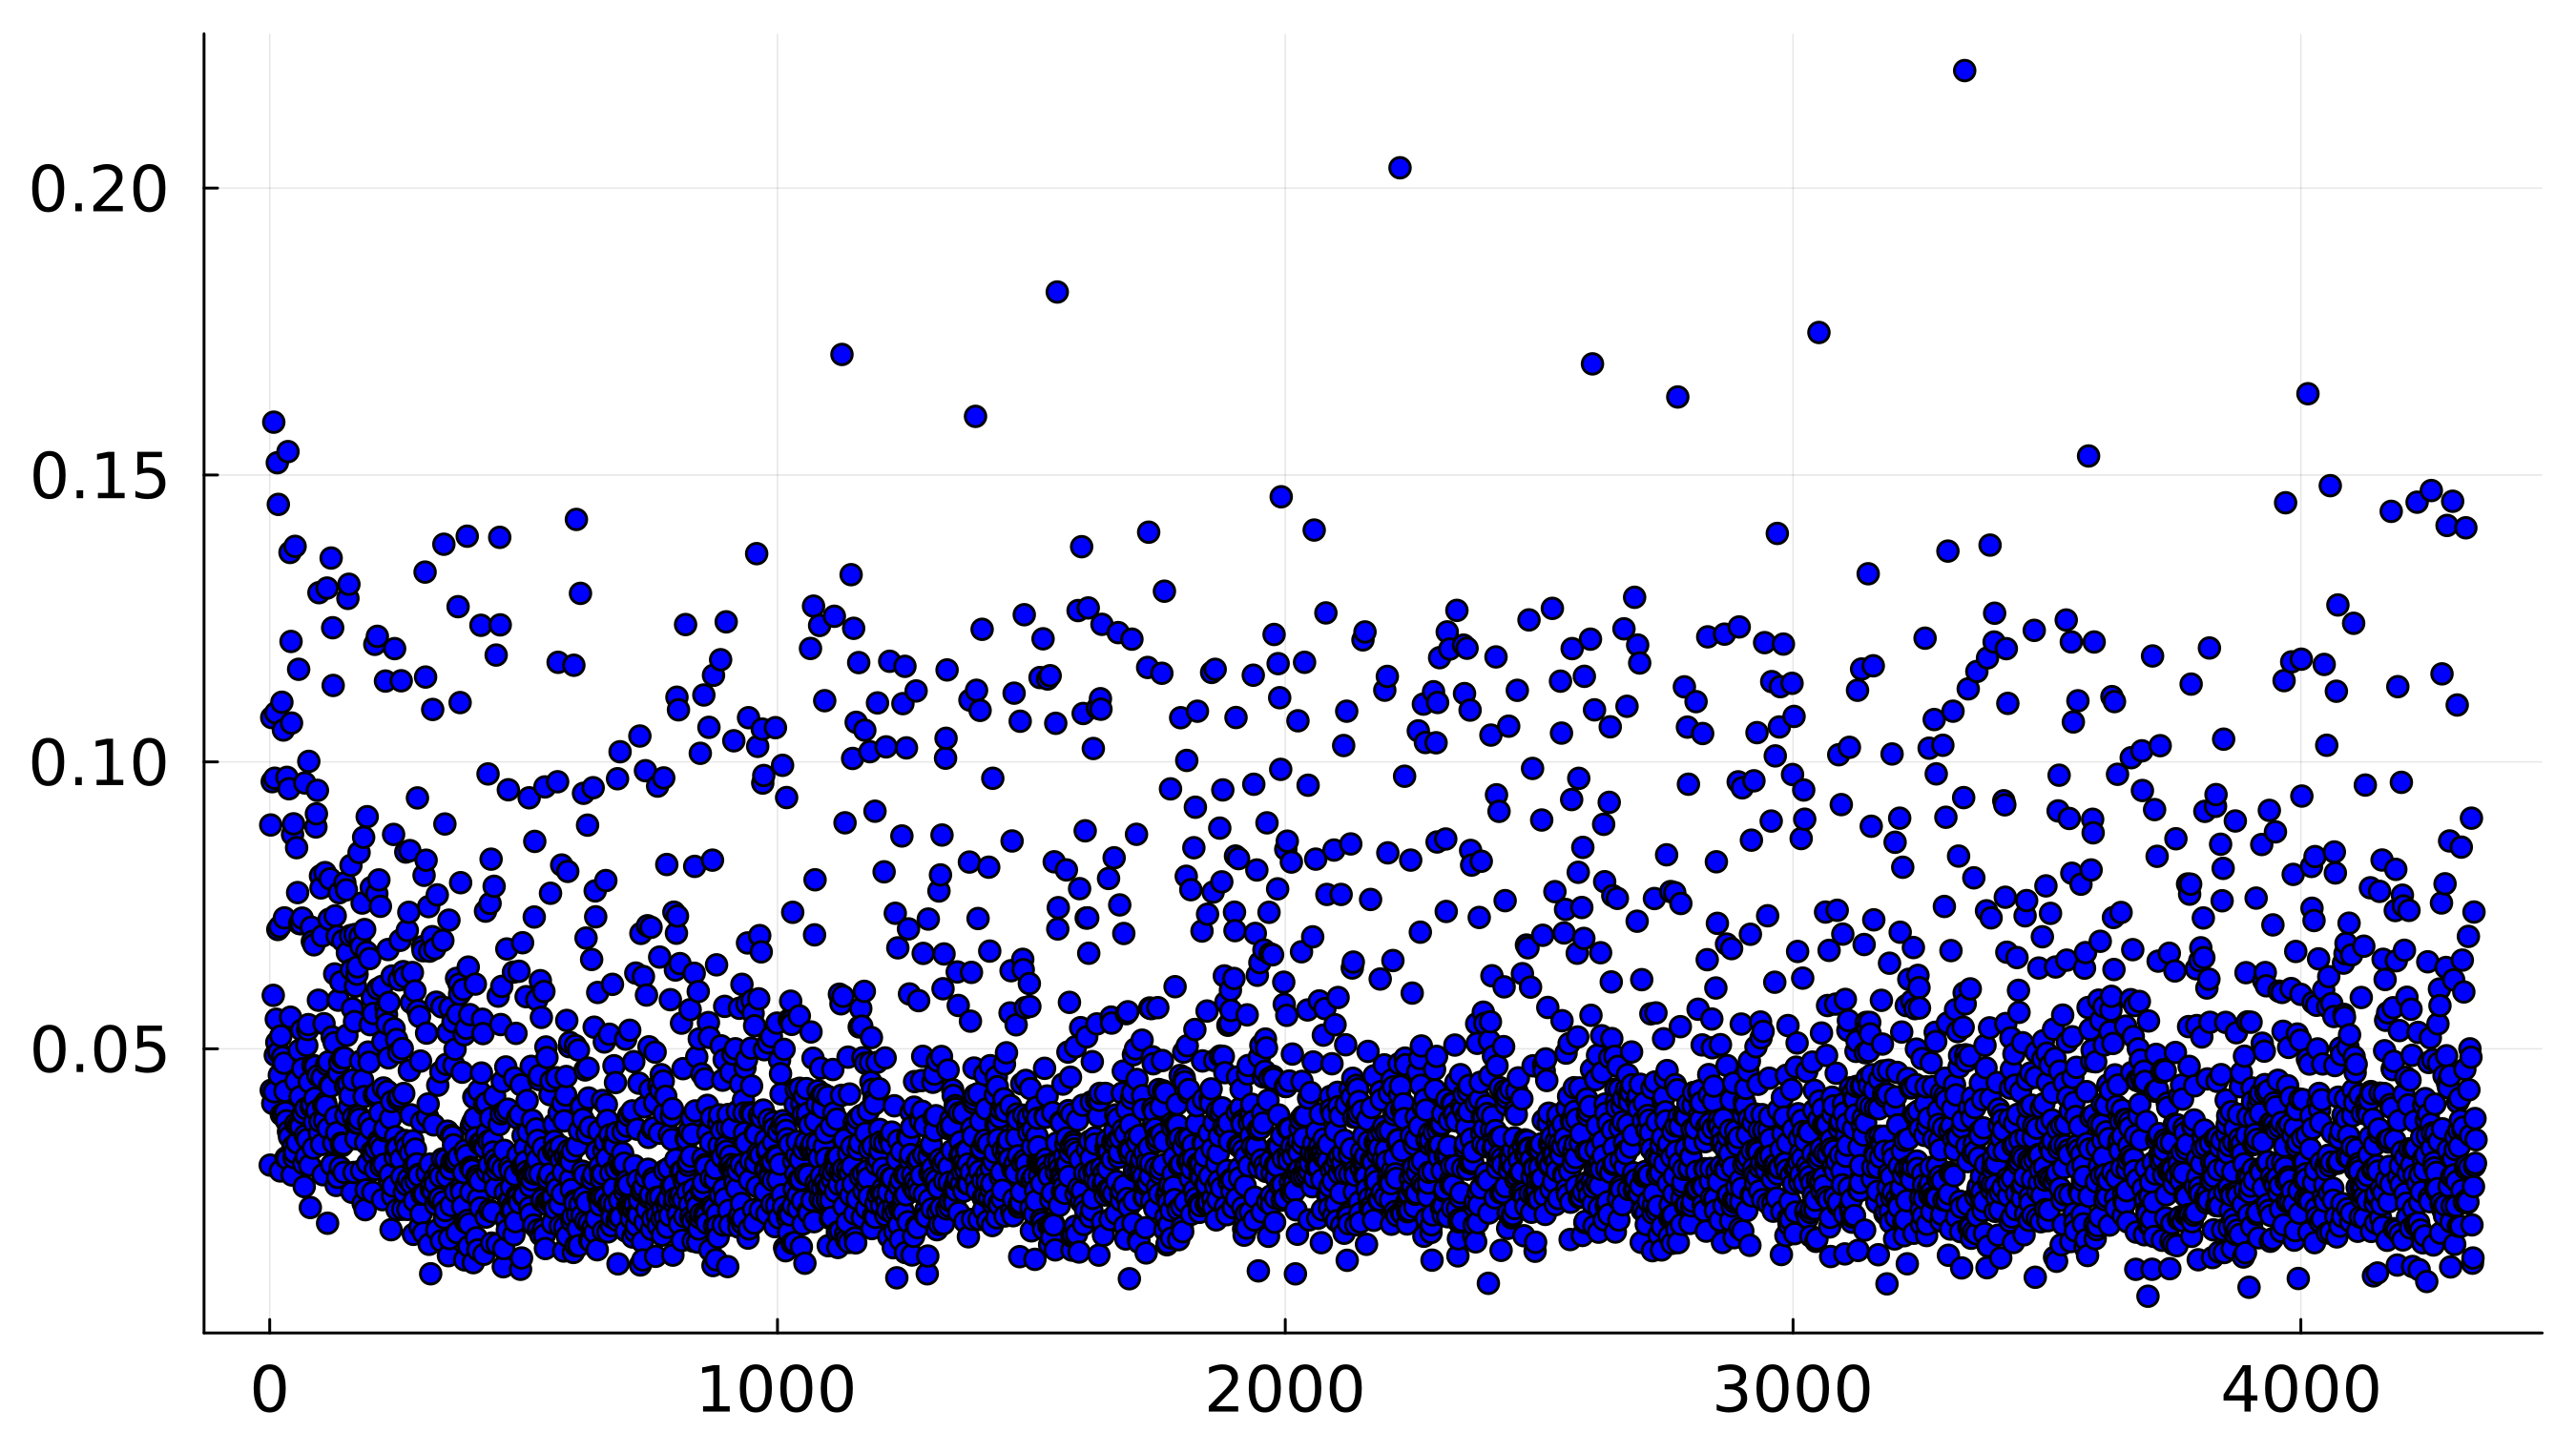
\includegraphics[width=\textwidth]{phalp_bow_rand_learning3}
        \caption{Embeddings using random amino acid vectors, made \textit{via} the bag-of-words embedding method}
        \label{fig:subfig-a2}
    \end{subfigure}
    \hfill
    \begin{subfigure}{0.48\textwidth}
        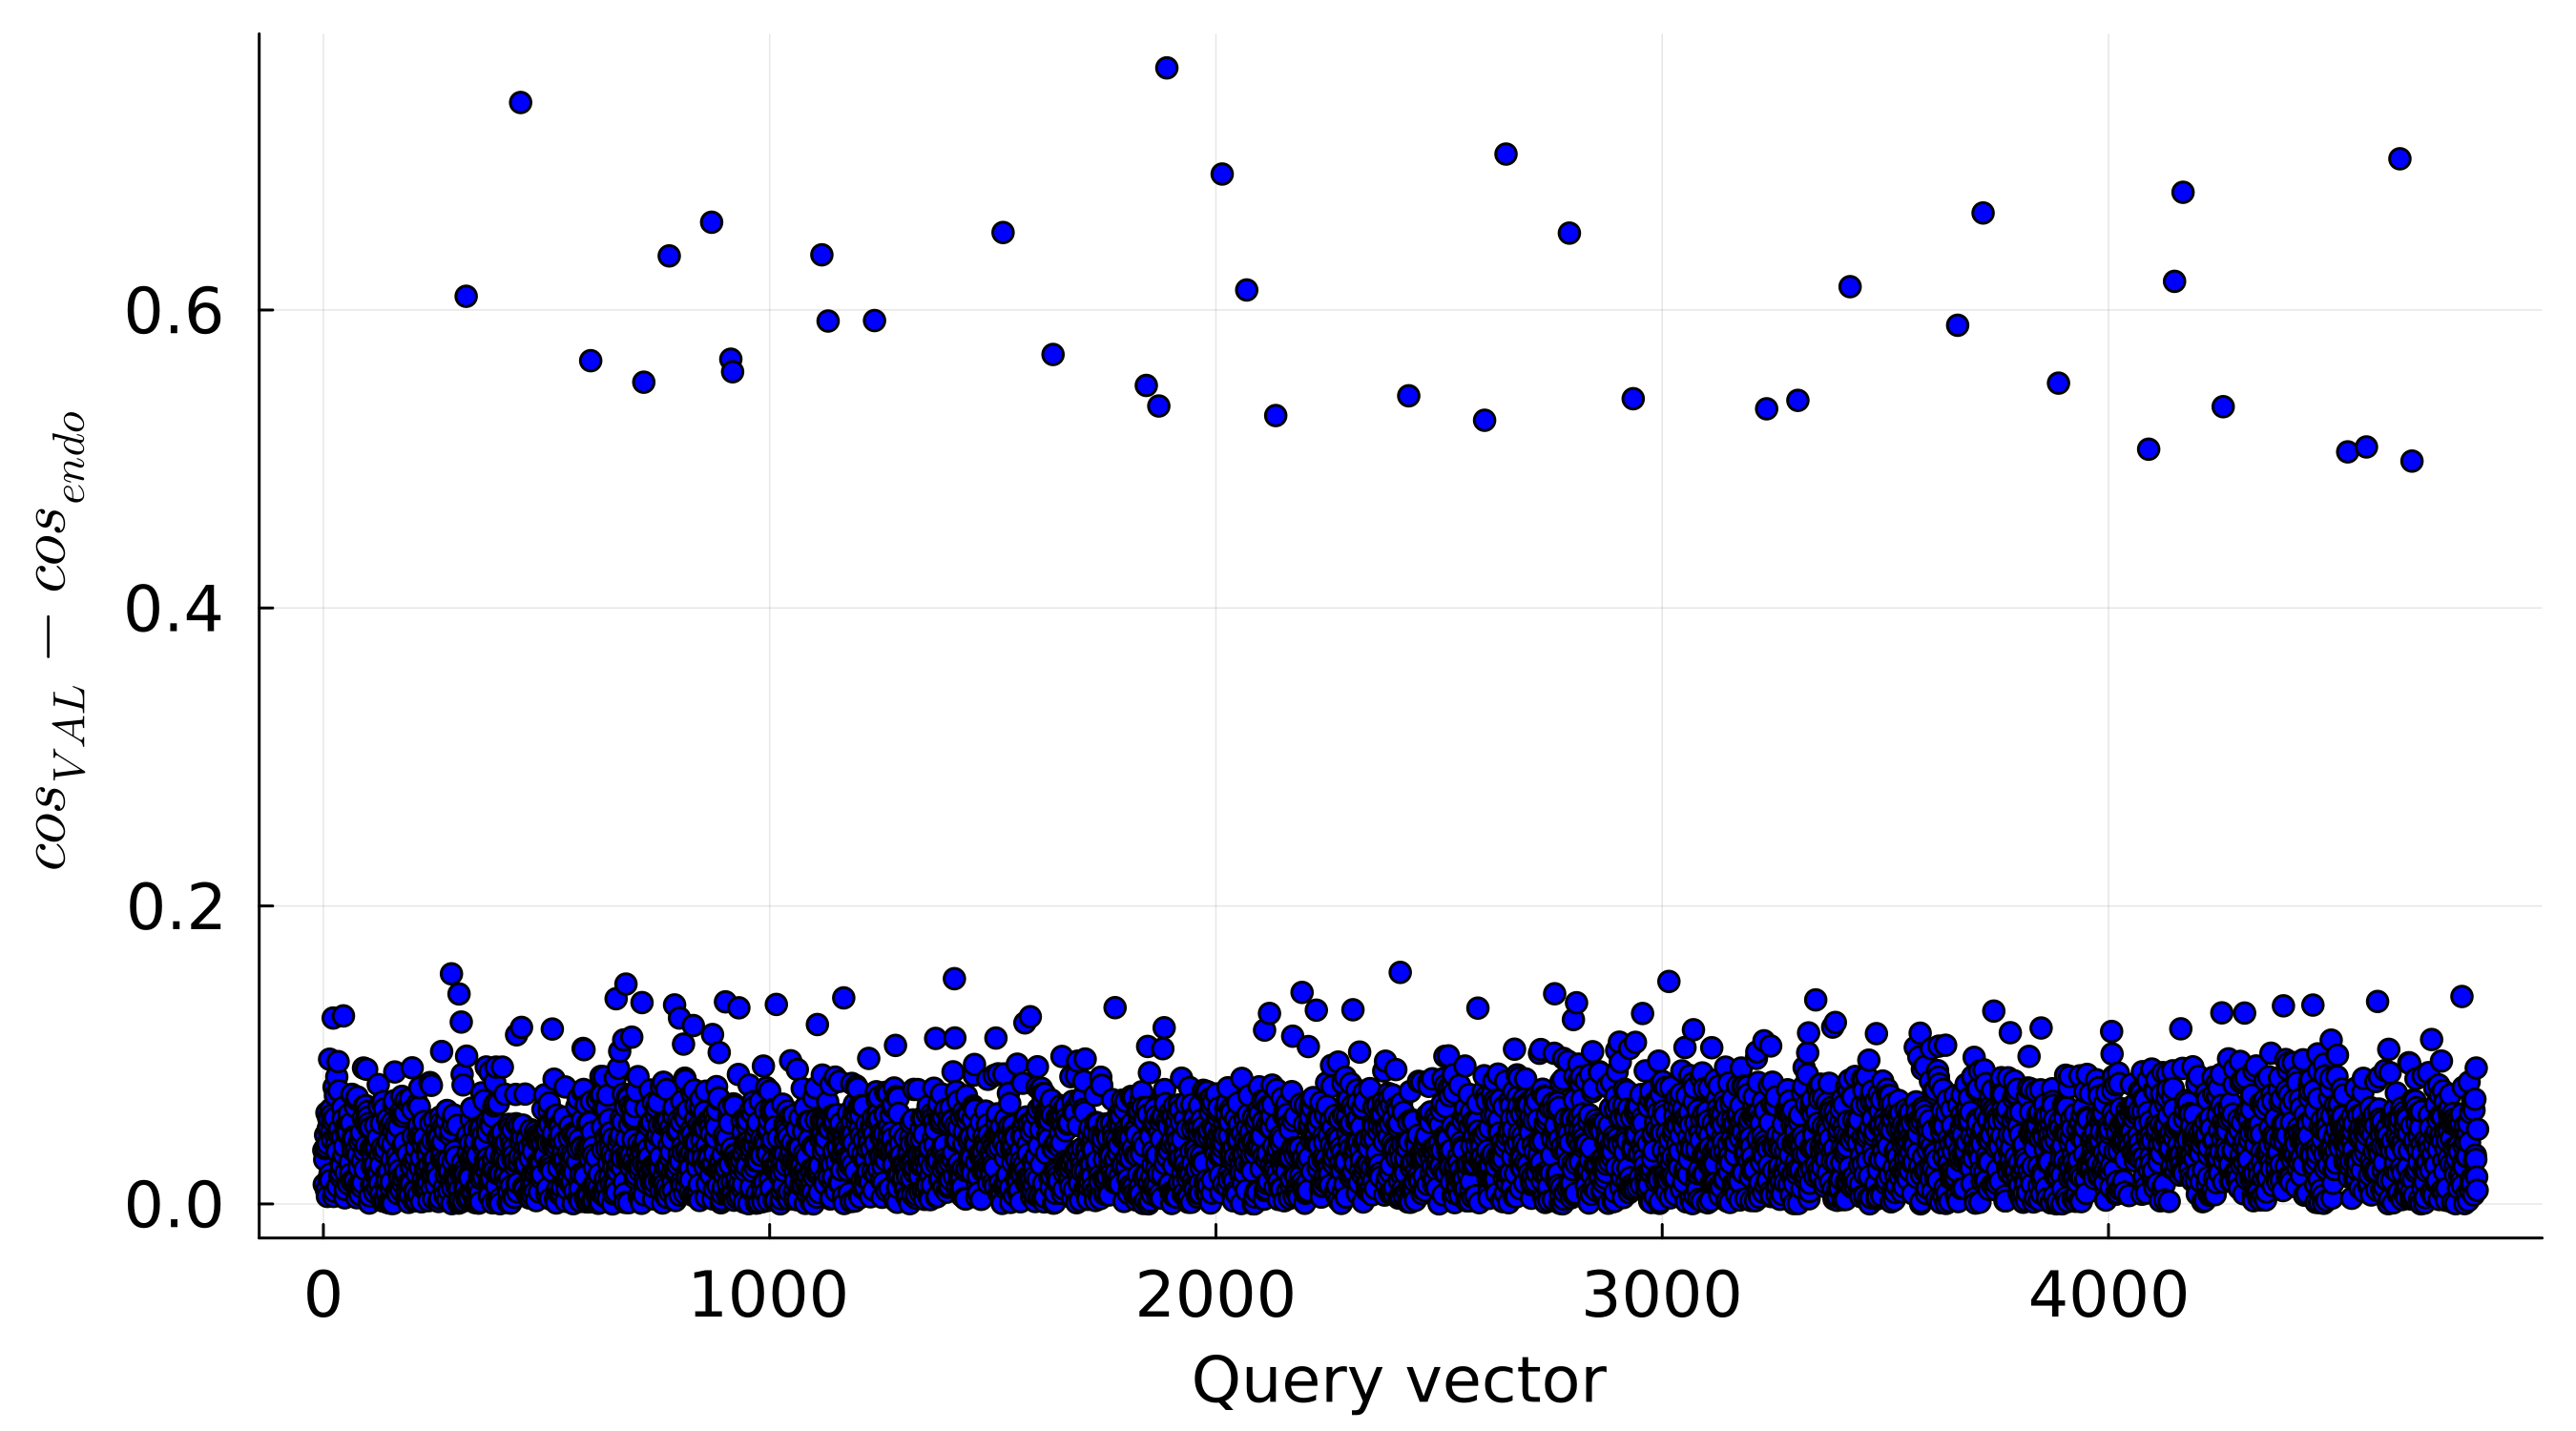
\includegraphics[width=\textwidth]{phalp_bow_esm_learning3}
        \caption{Embeddings using projected ESM-2 amino acid vectors, made \textit{via} the bag-of-words embedding method}
        \label{fig:subfig-b2}
    \end{subfigure}
    
    \begin{subfigure}{0.48\textwidth}
        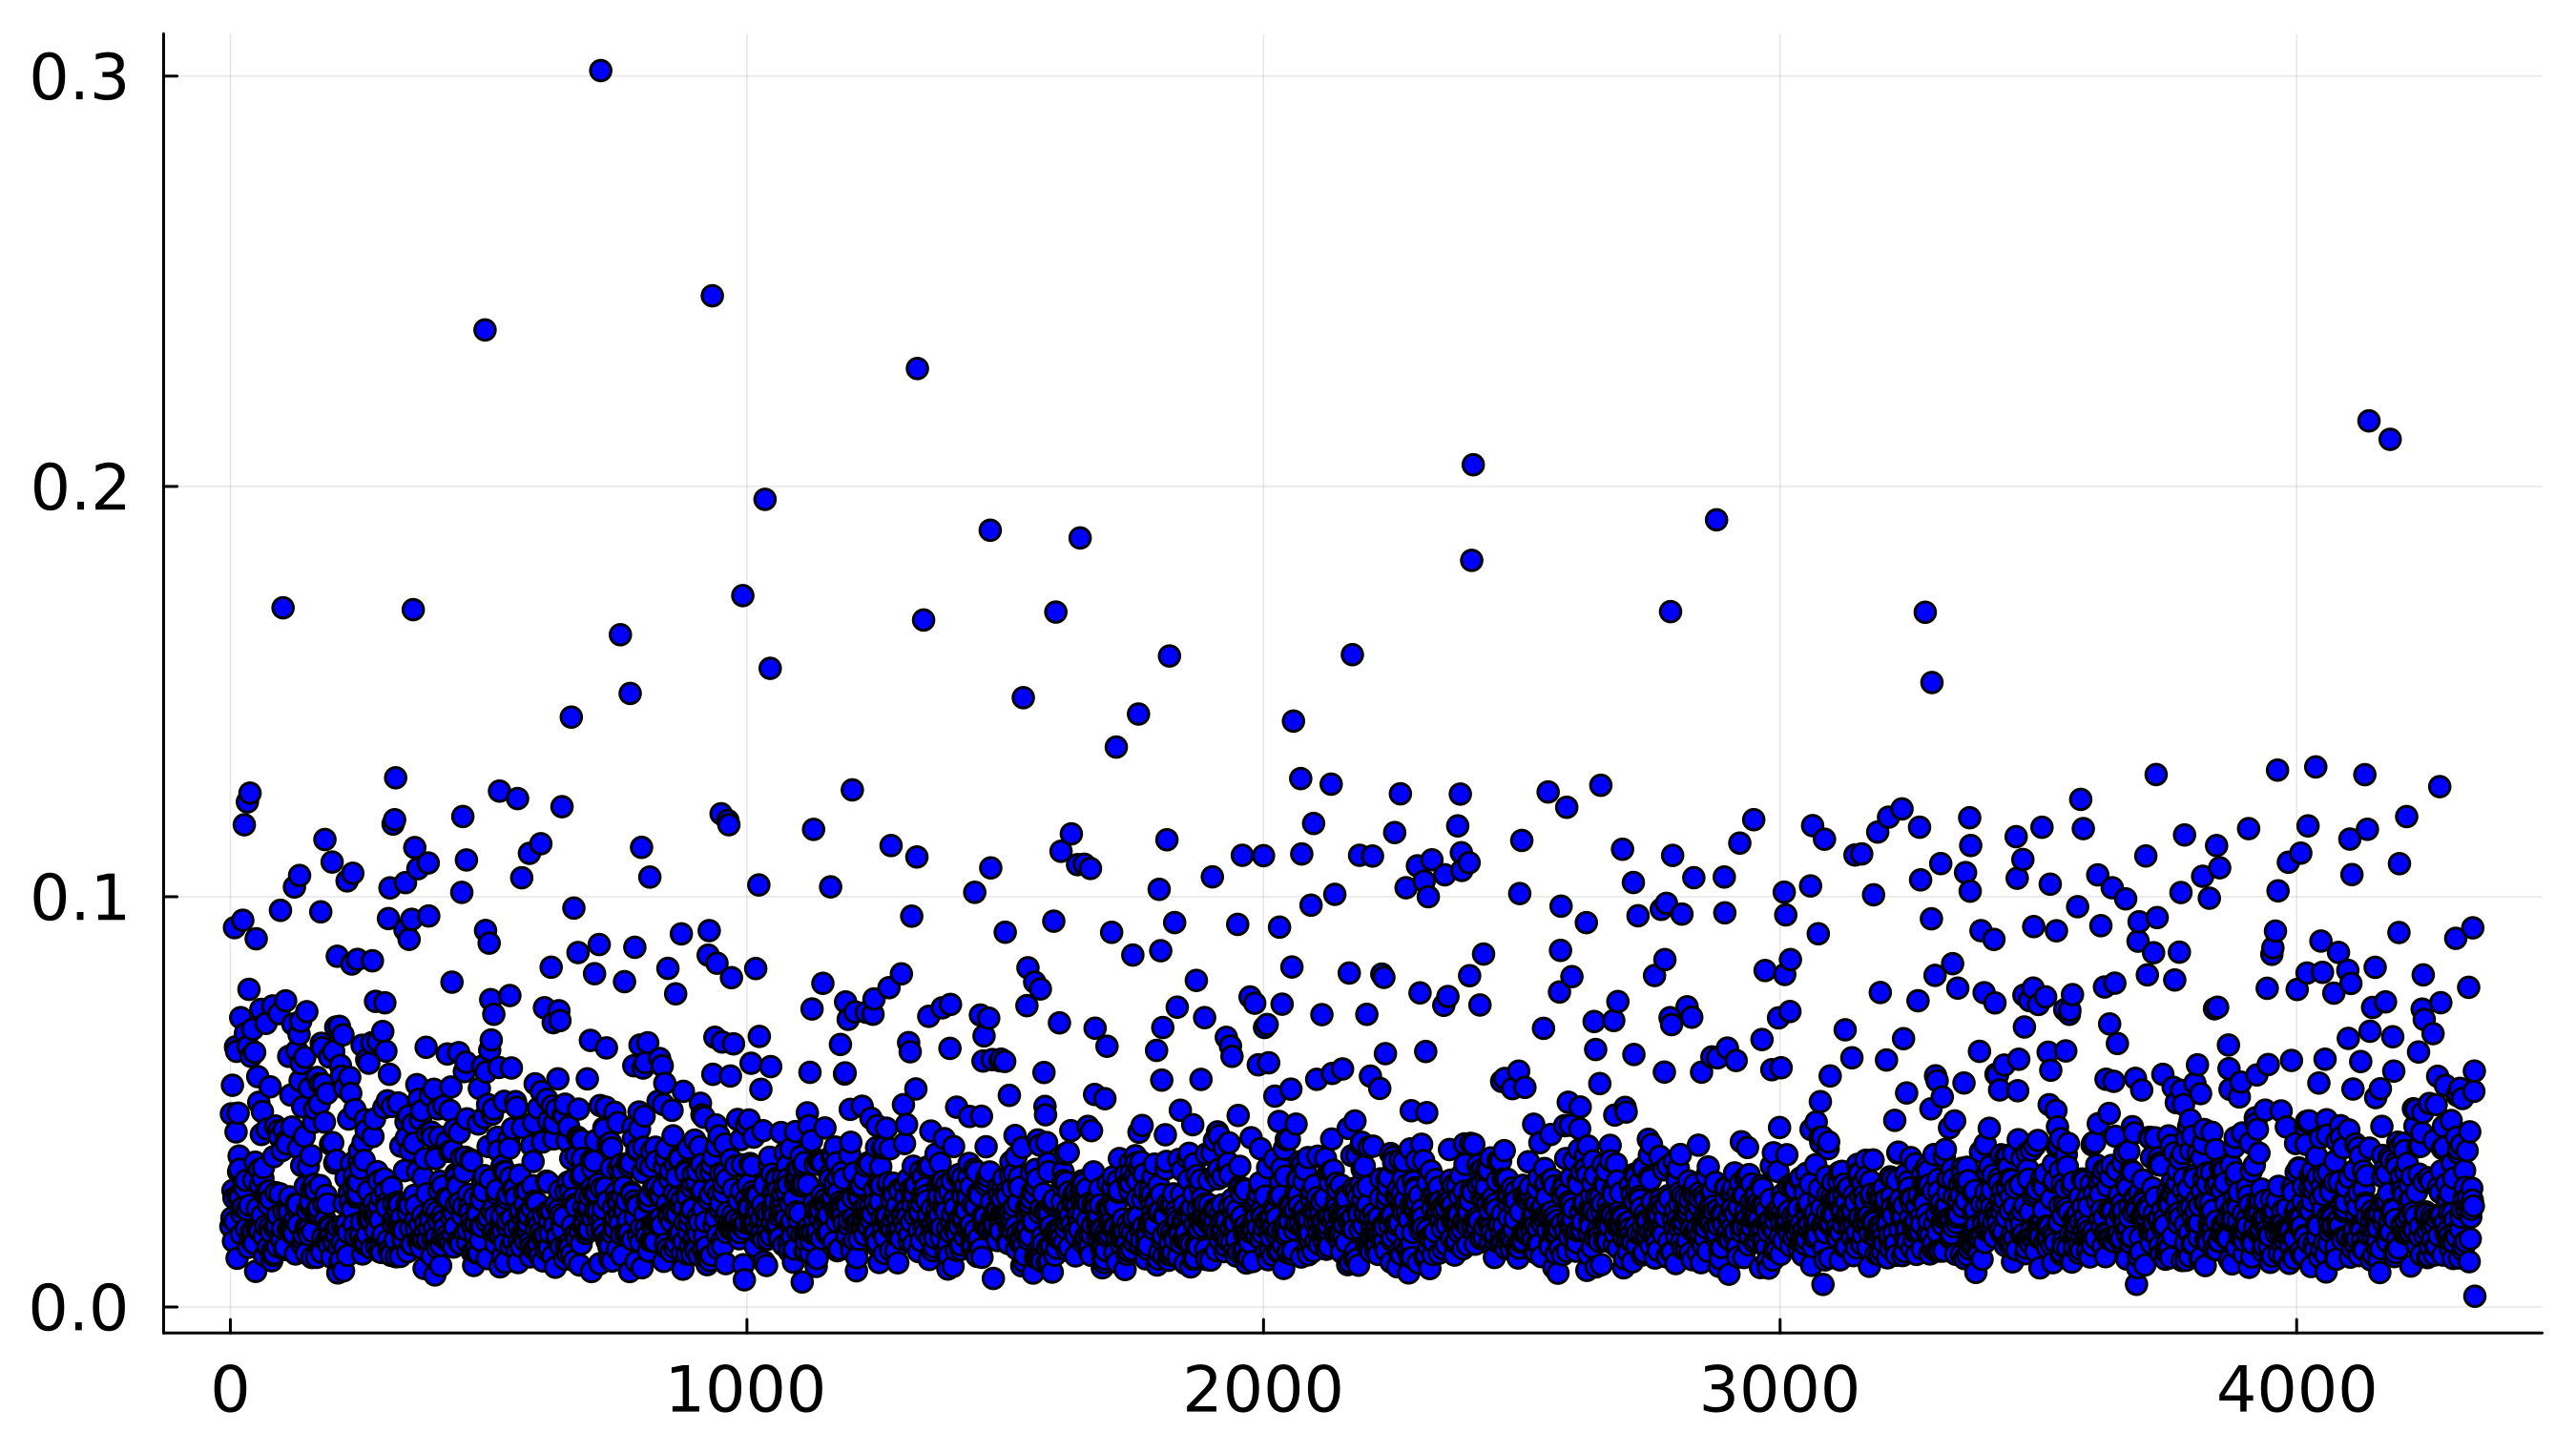
\includegraphics[width=\textwidth]{phalp_cnn_rand_learning3}
        \caption{Embeddings using random amino acid vectors, made \textit{via} the convolutional embedding method}
        \label{fig:subfig-c2}
    \end{subfigure}
    \hfill
    \begin{subfigure}{0.48\textwidth}
        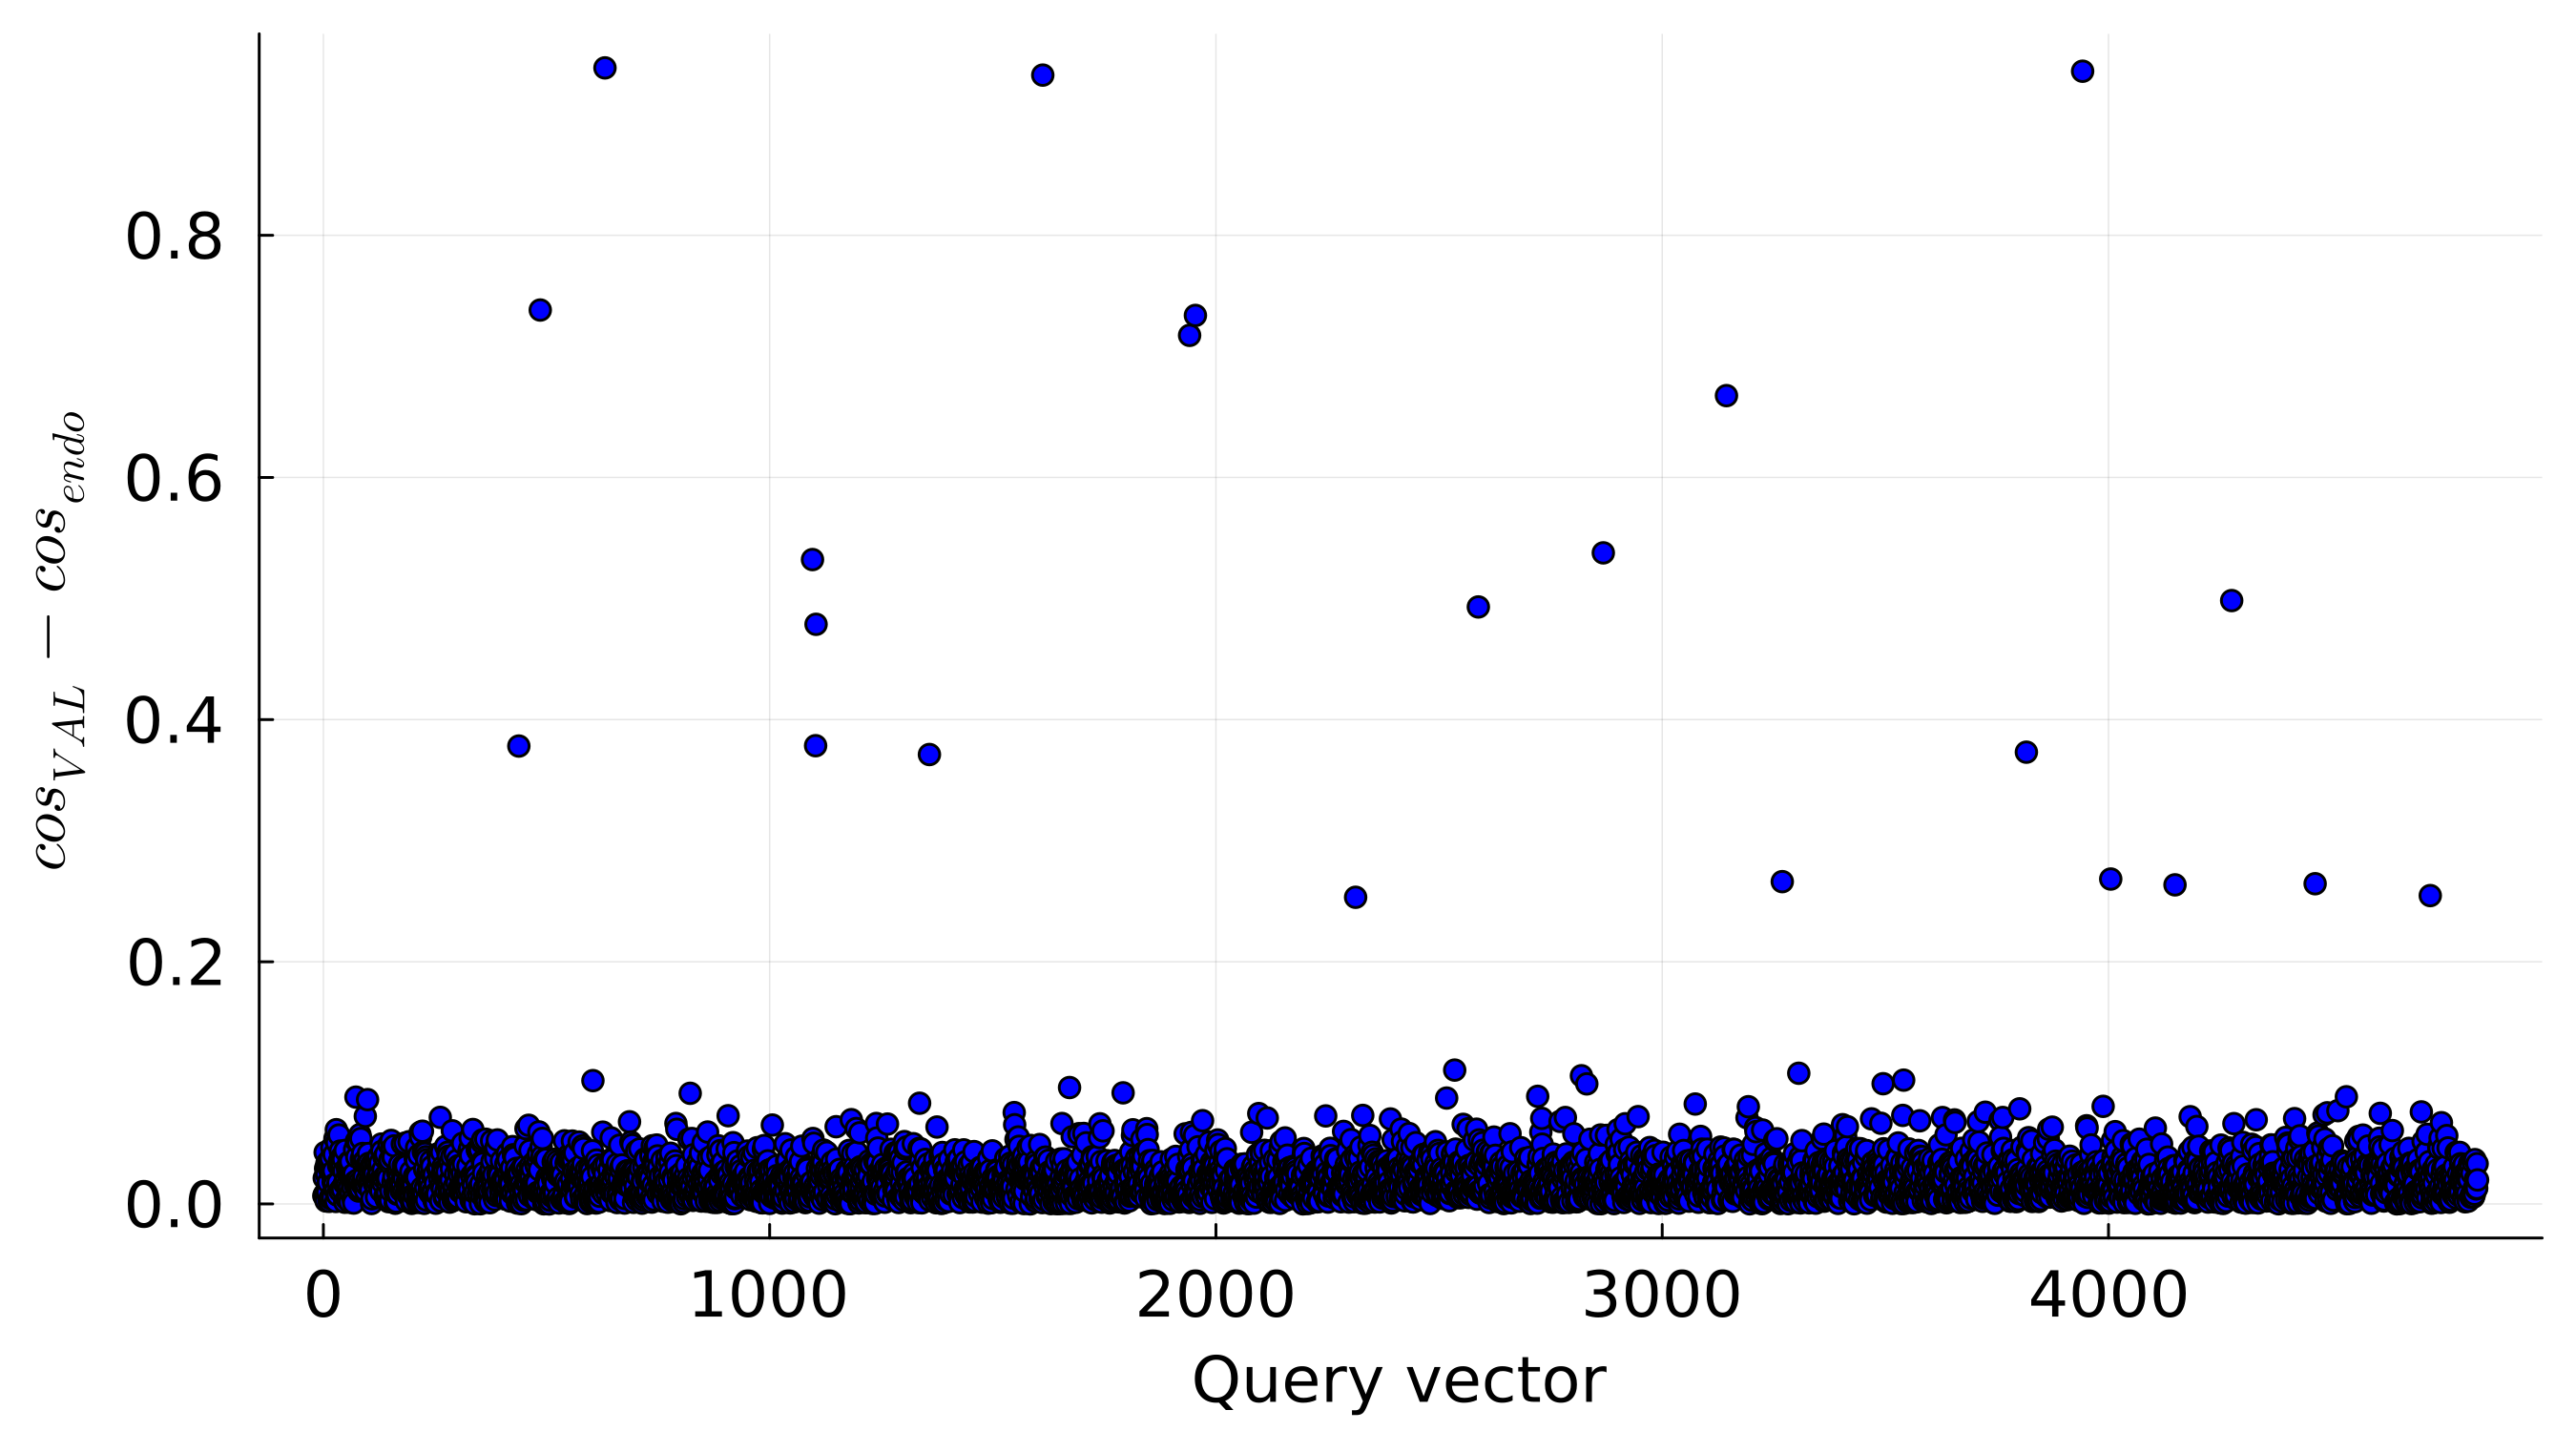
\includegraphics[width=\textwidth]{phalp_cnn_esm_learning3}
        \caption{Embeddings using projected ESM-2 acid vectors, made \textit{via} the convolutional embedding method}
        \label{fig:subfig-d2}
    \end{subfigure}
    \caption{Absolute difference between the cosine similarity of the query vector with the VAL class vector and the cosine similarity of the query vector with the endolysin class vector before the weighted update while following the OnlineHD single-pass training procedure. Trained using hyperdimensional embeddings from all protein sequences in the PhaLP dataset whose types were manually annotated.}
    \label{fig:main2}
\end{figure}

To further research the power of OnlineHD, we aim to monitor its training procedure when applied to the PhaLP dataset. We calculate the absolute difference between the cosine similarities, $cos(V, C_{VAL})$ and $cos(V, C_{endo})$, as described in equations 4.3 and 4.4. By observing this metric, we can gain insights into the behavior of the hyperdimensional vectors in the OnlineHD model during training. A possibility to expect is that the difference in cosine similarities increases throughout the training procedure as the model learns to differentiate the two classes. However, these differences don't increase noticeably in this case as shown in Figure~\ref{fig:main2}.

\begin{figure}[ht!]
    \centering
    \begin{subfigure}{0.48\textwidth}
        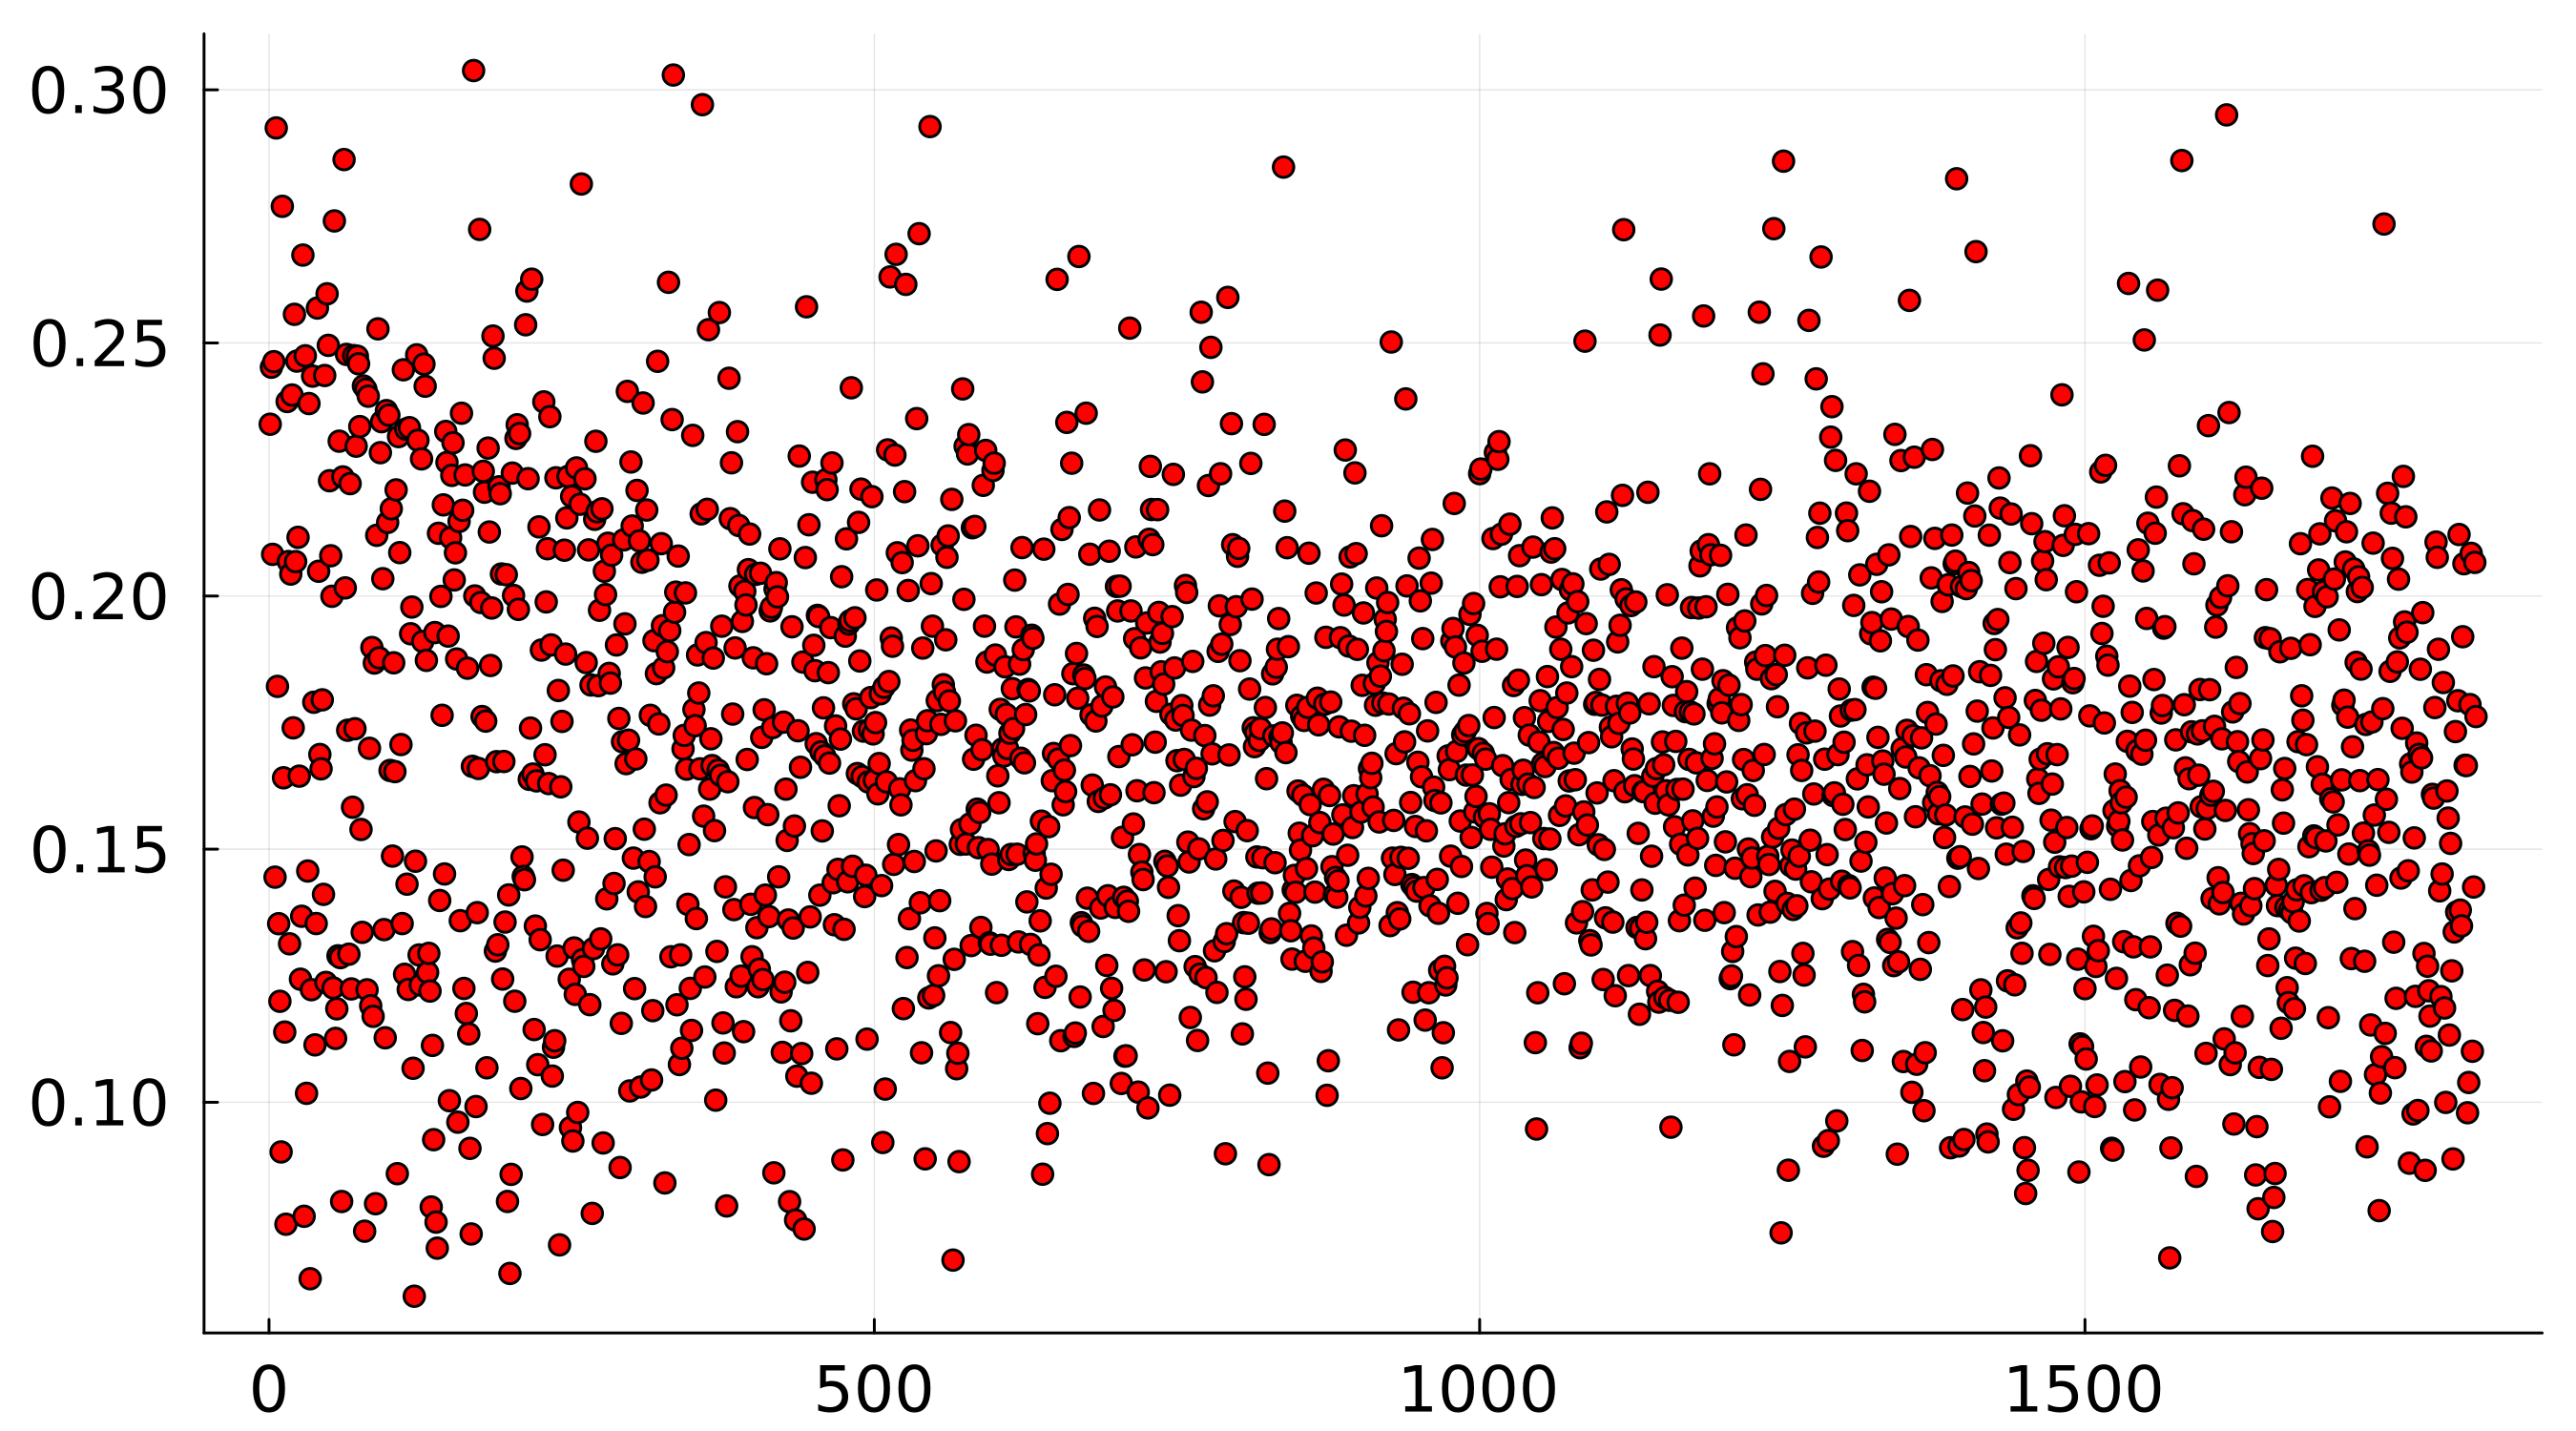
\includegraphics[width=\textwidth]{phalp_bow_rand_learningV}
        \caption{VALs embedded using random amino acid vectors \textit{via} the bag-of-words method}
        \label{fig:subfig-a}
    \end{subfigure}
    \hfill
    \begin{subfigure}{0.48\textwidth}
        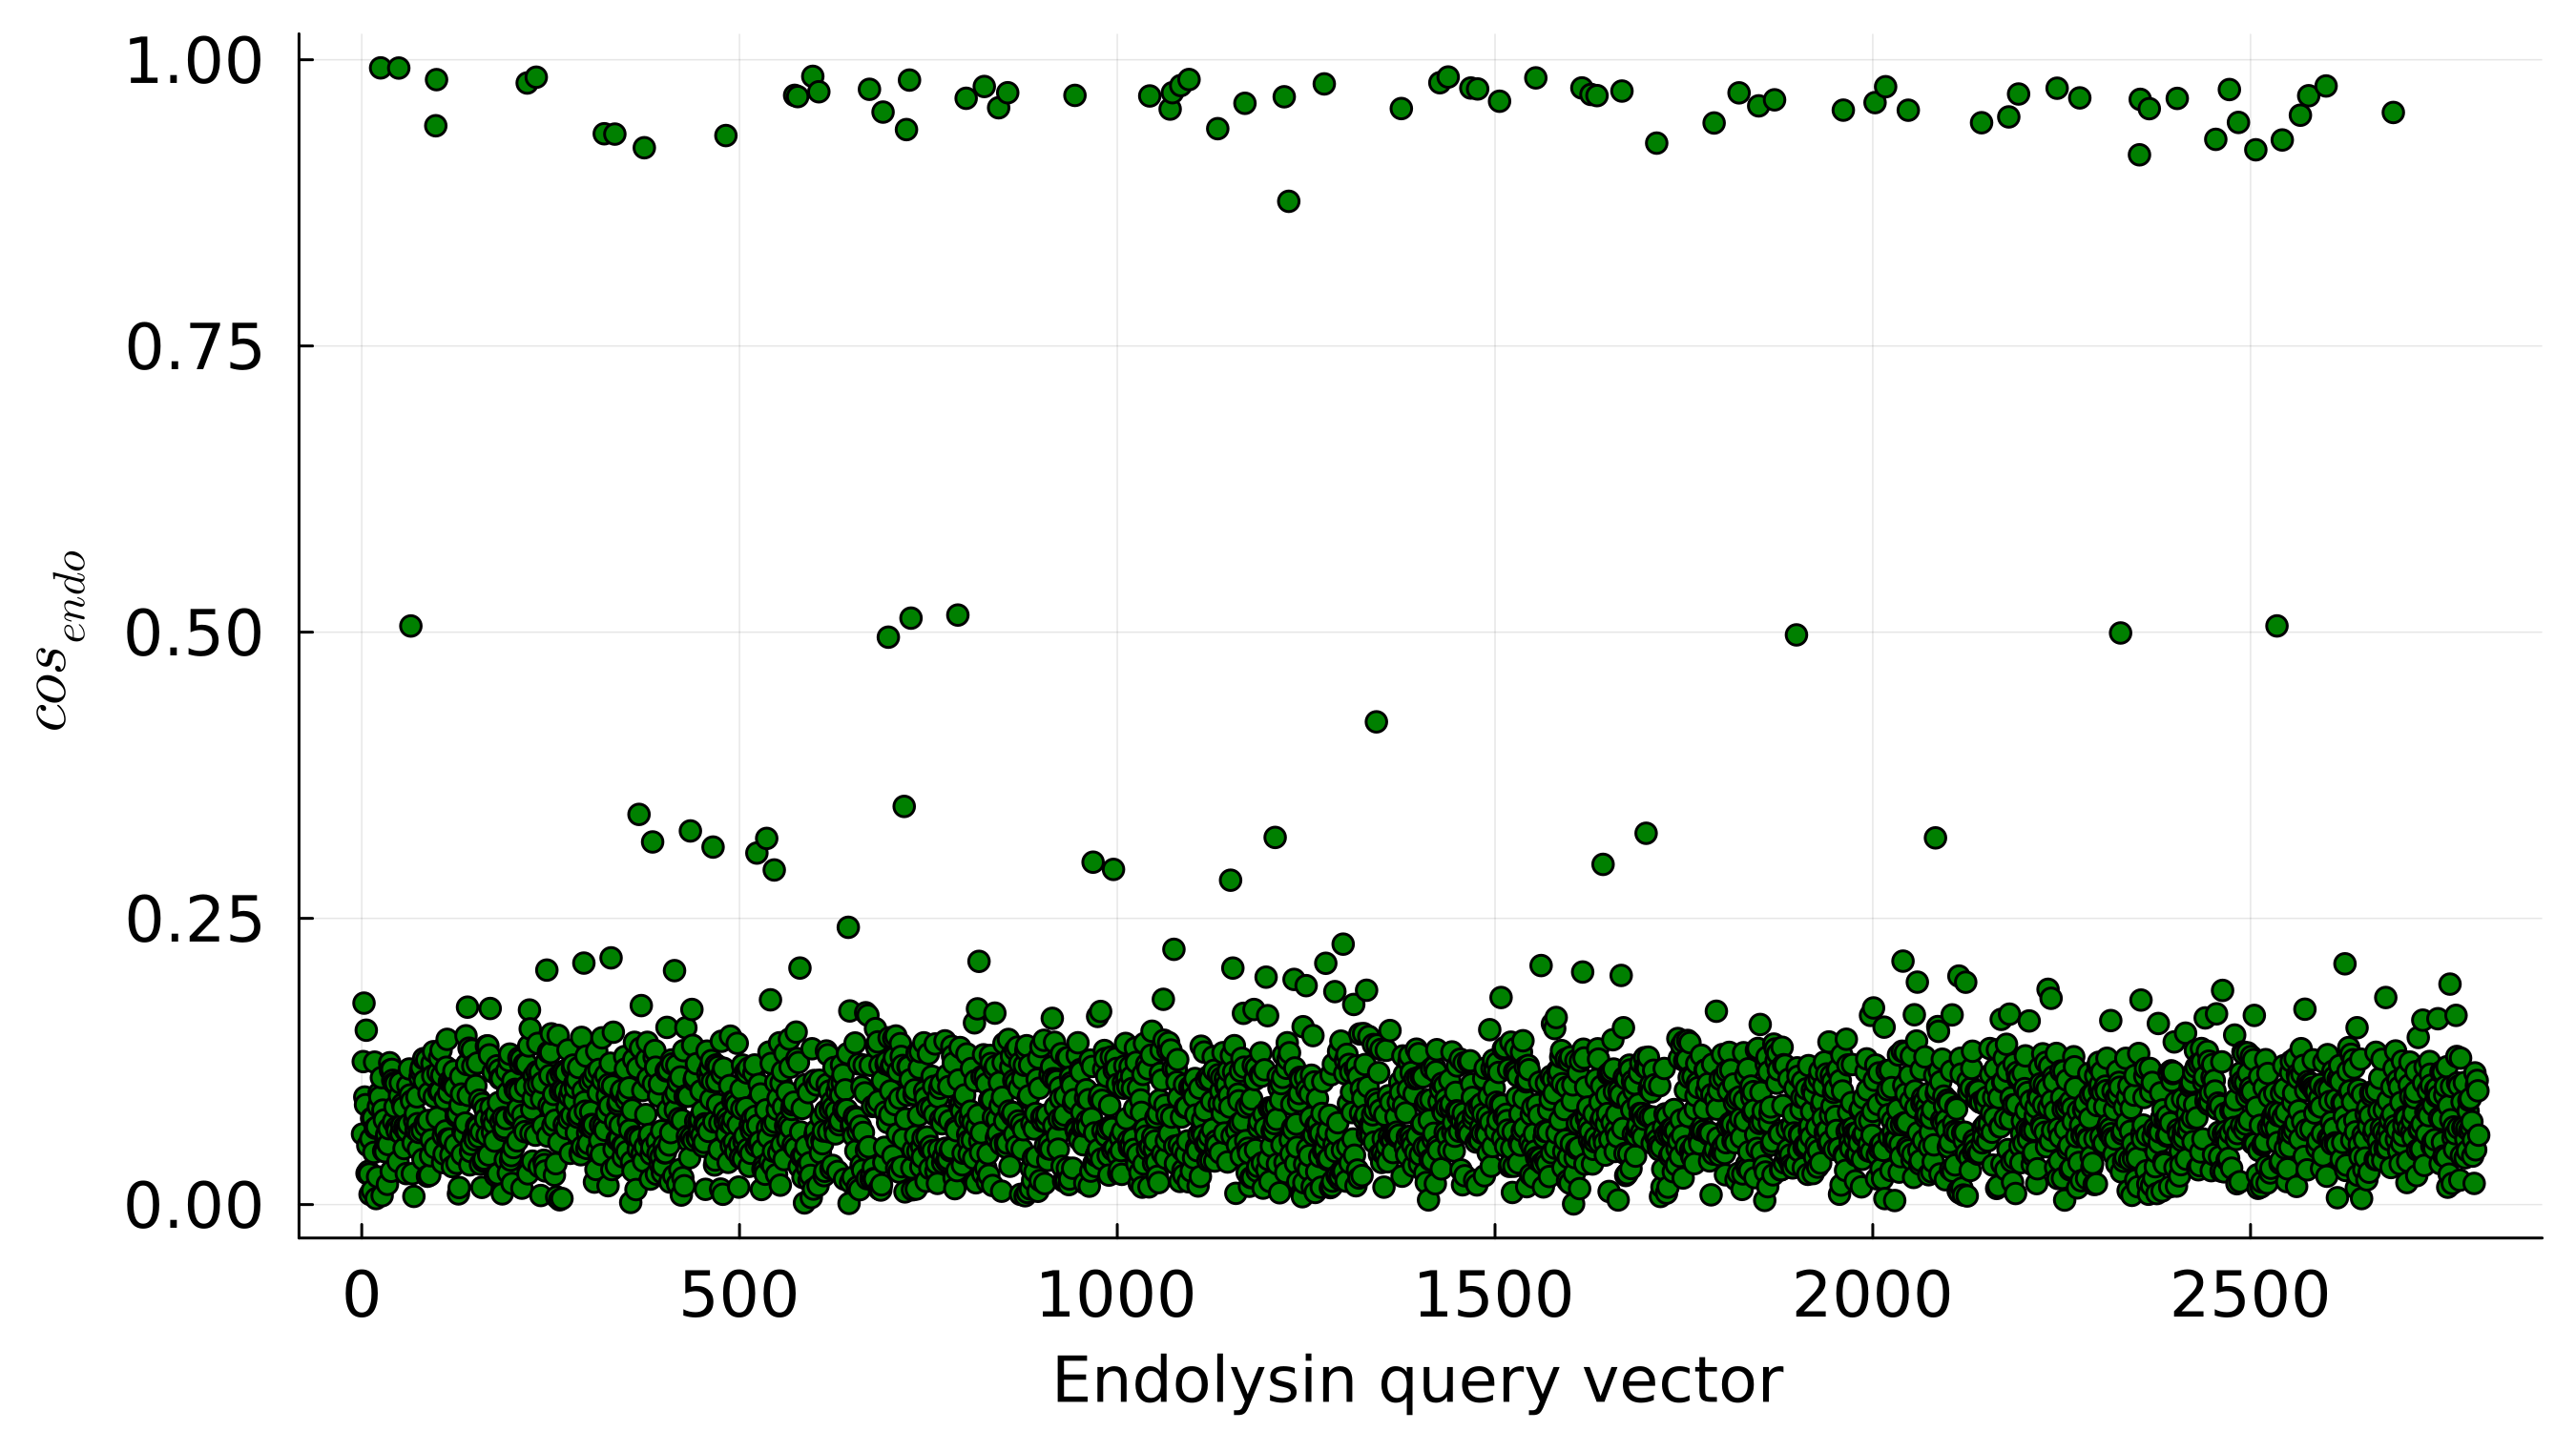
\includegraphics[width=\textwidth]{phalp_bow_rand_learningE}
        \caption{Endolysins embedded using random amino acid vectors \textit{via} the bag-of-words embedding method}
        \label{fig:subfig-b}
    \end{subfigure}
    
    \begin{subfigure}{0.48\textwidth}
        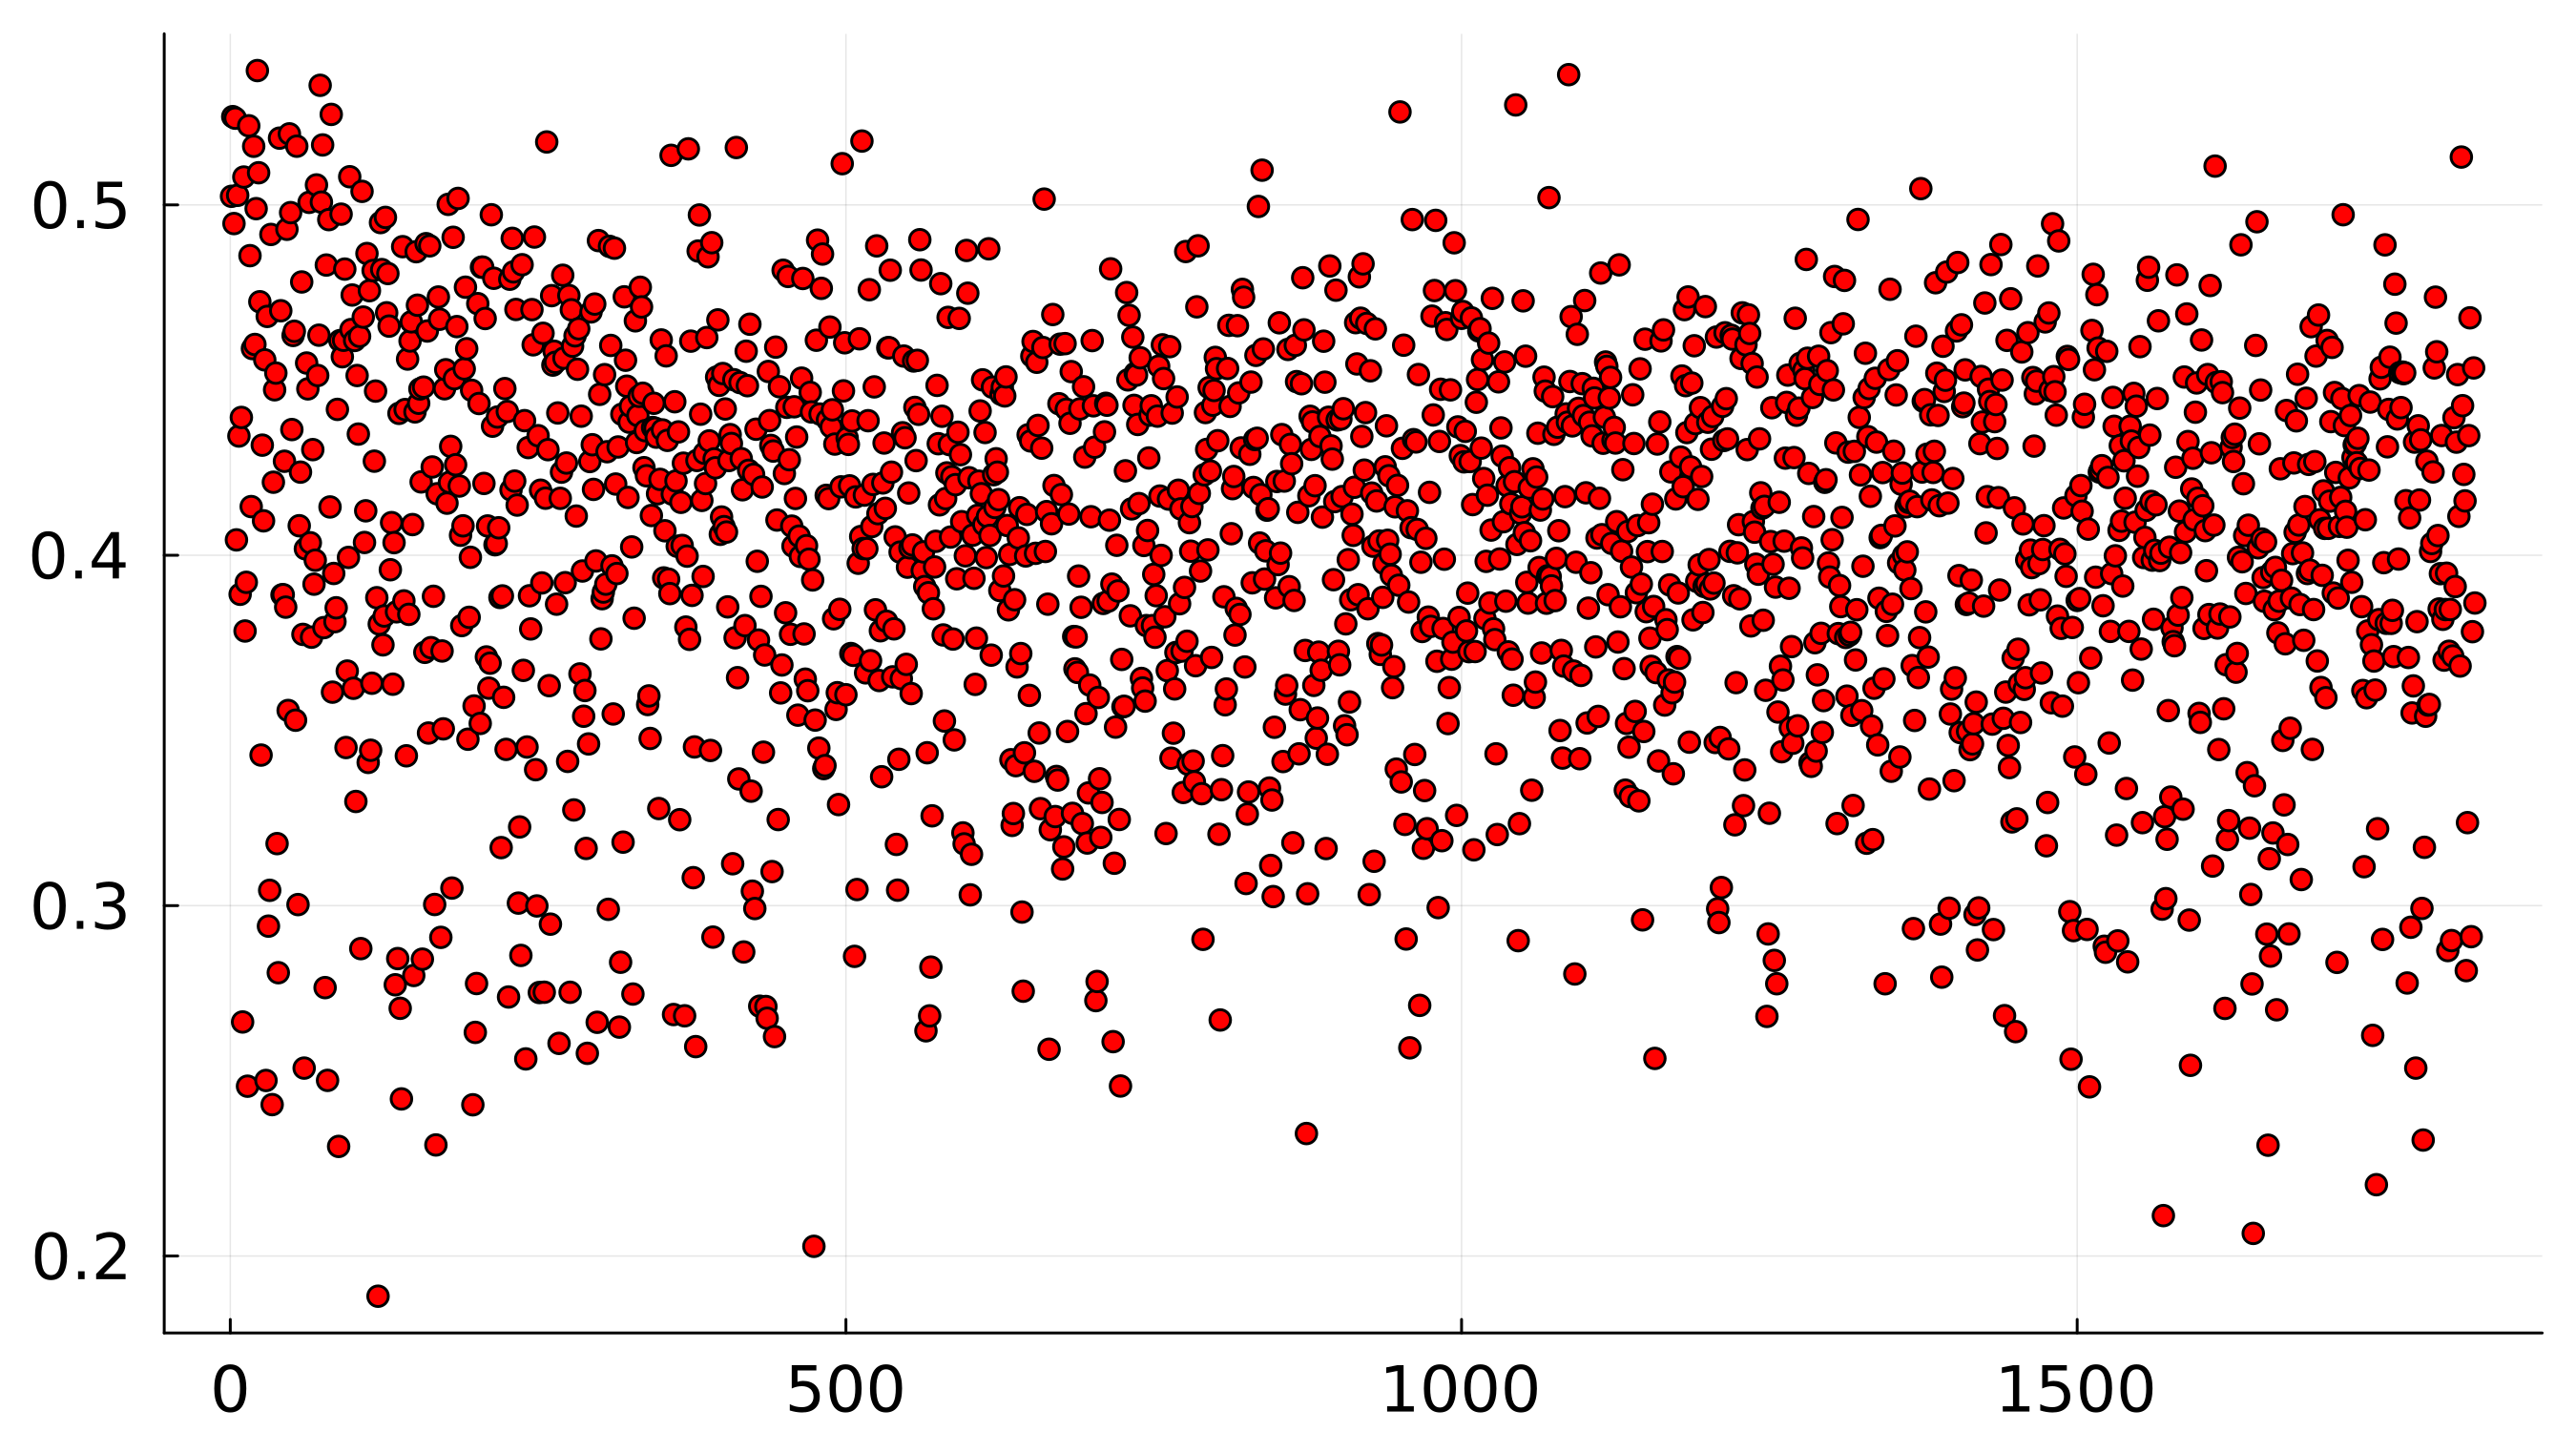
\includegraphics[width=\textwidth]{phalp_bow_esm_learningV}
        \caption{VALs embedded using projected ESM-2 amino acid vectors \textit{via} the bag-of-words embedding method}
        \label{fig:subfig-c}
    \end{subfigure}
    \hfill
    \begin{subfigure}{0.48\textwidth}
        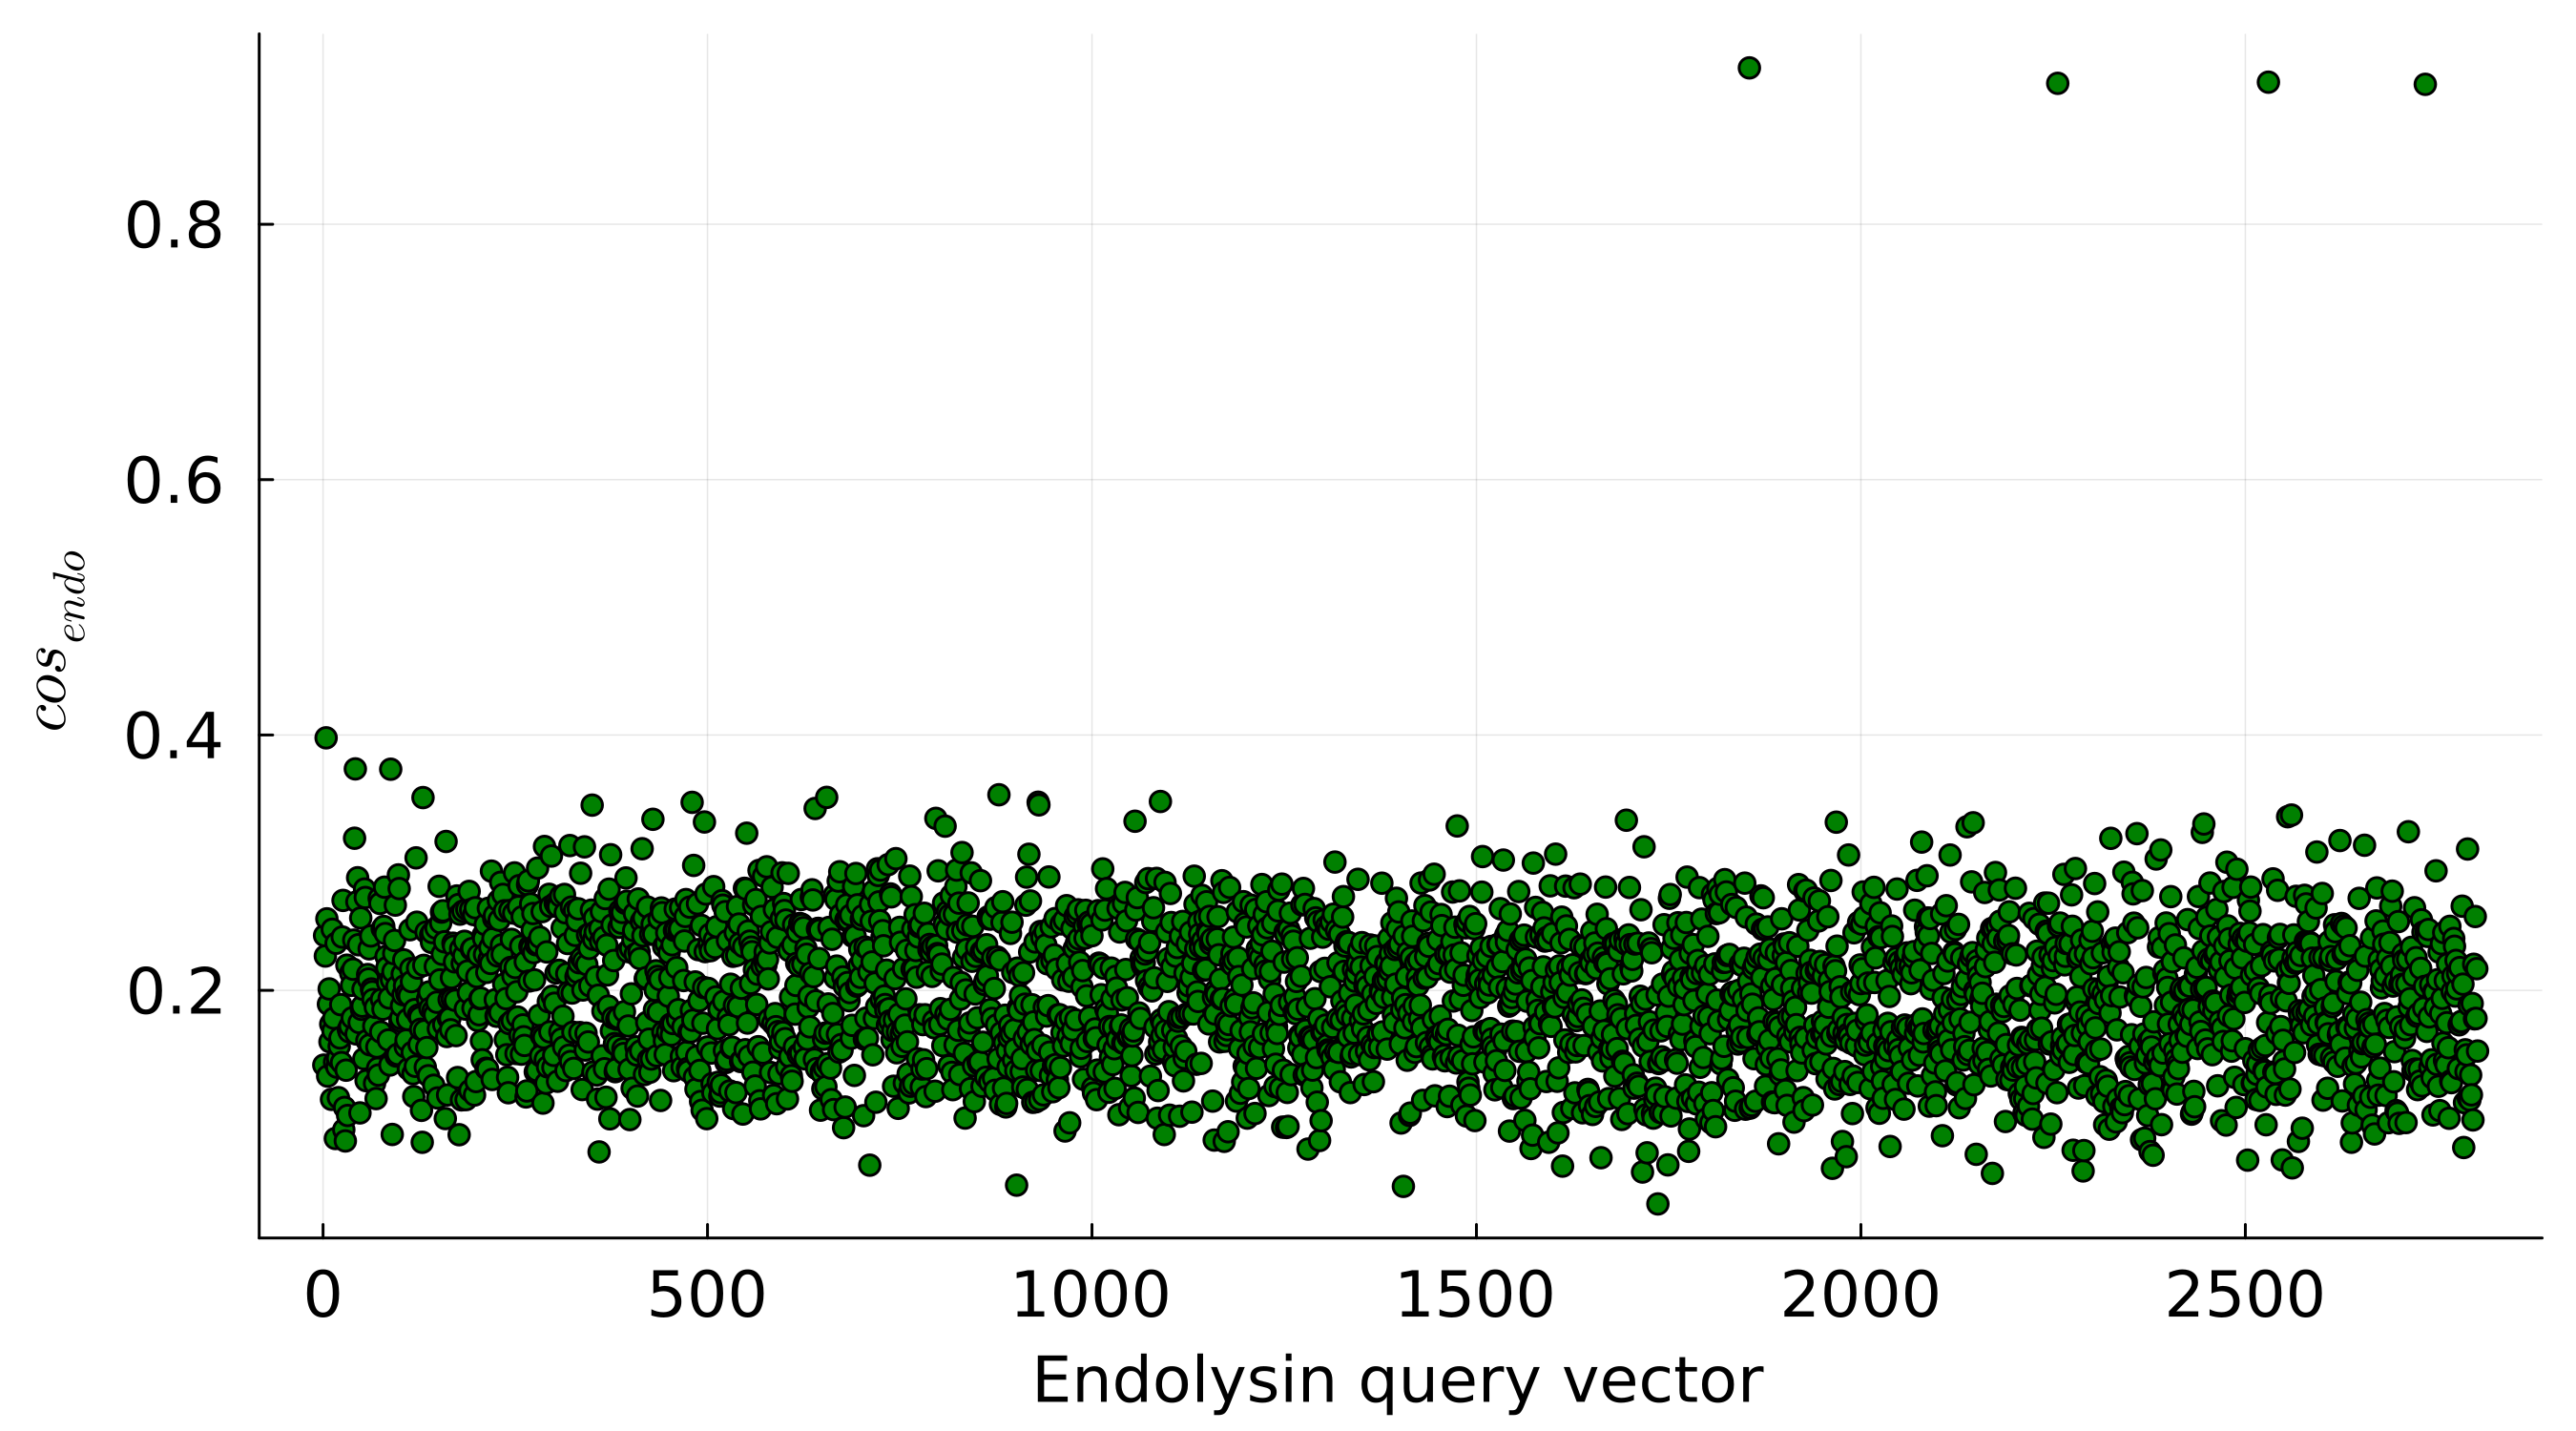
\includegraphics[width=\textwidth]{phalp_bow_esm_learningE}
        \caption{Endolysins embedded using projected ESM-2 amino acid vectors \textit{via} the bag-of-words embedding method}
        \label{fig:subfig-d}
    \end{subfigure}
    
    \begin{subfigure}{0.48\textwidth}
        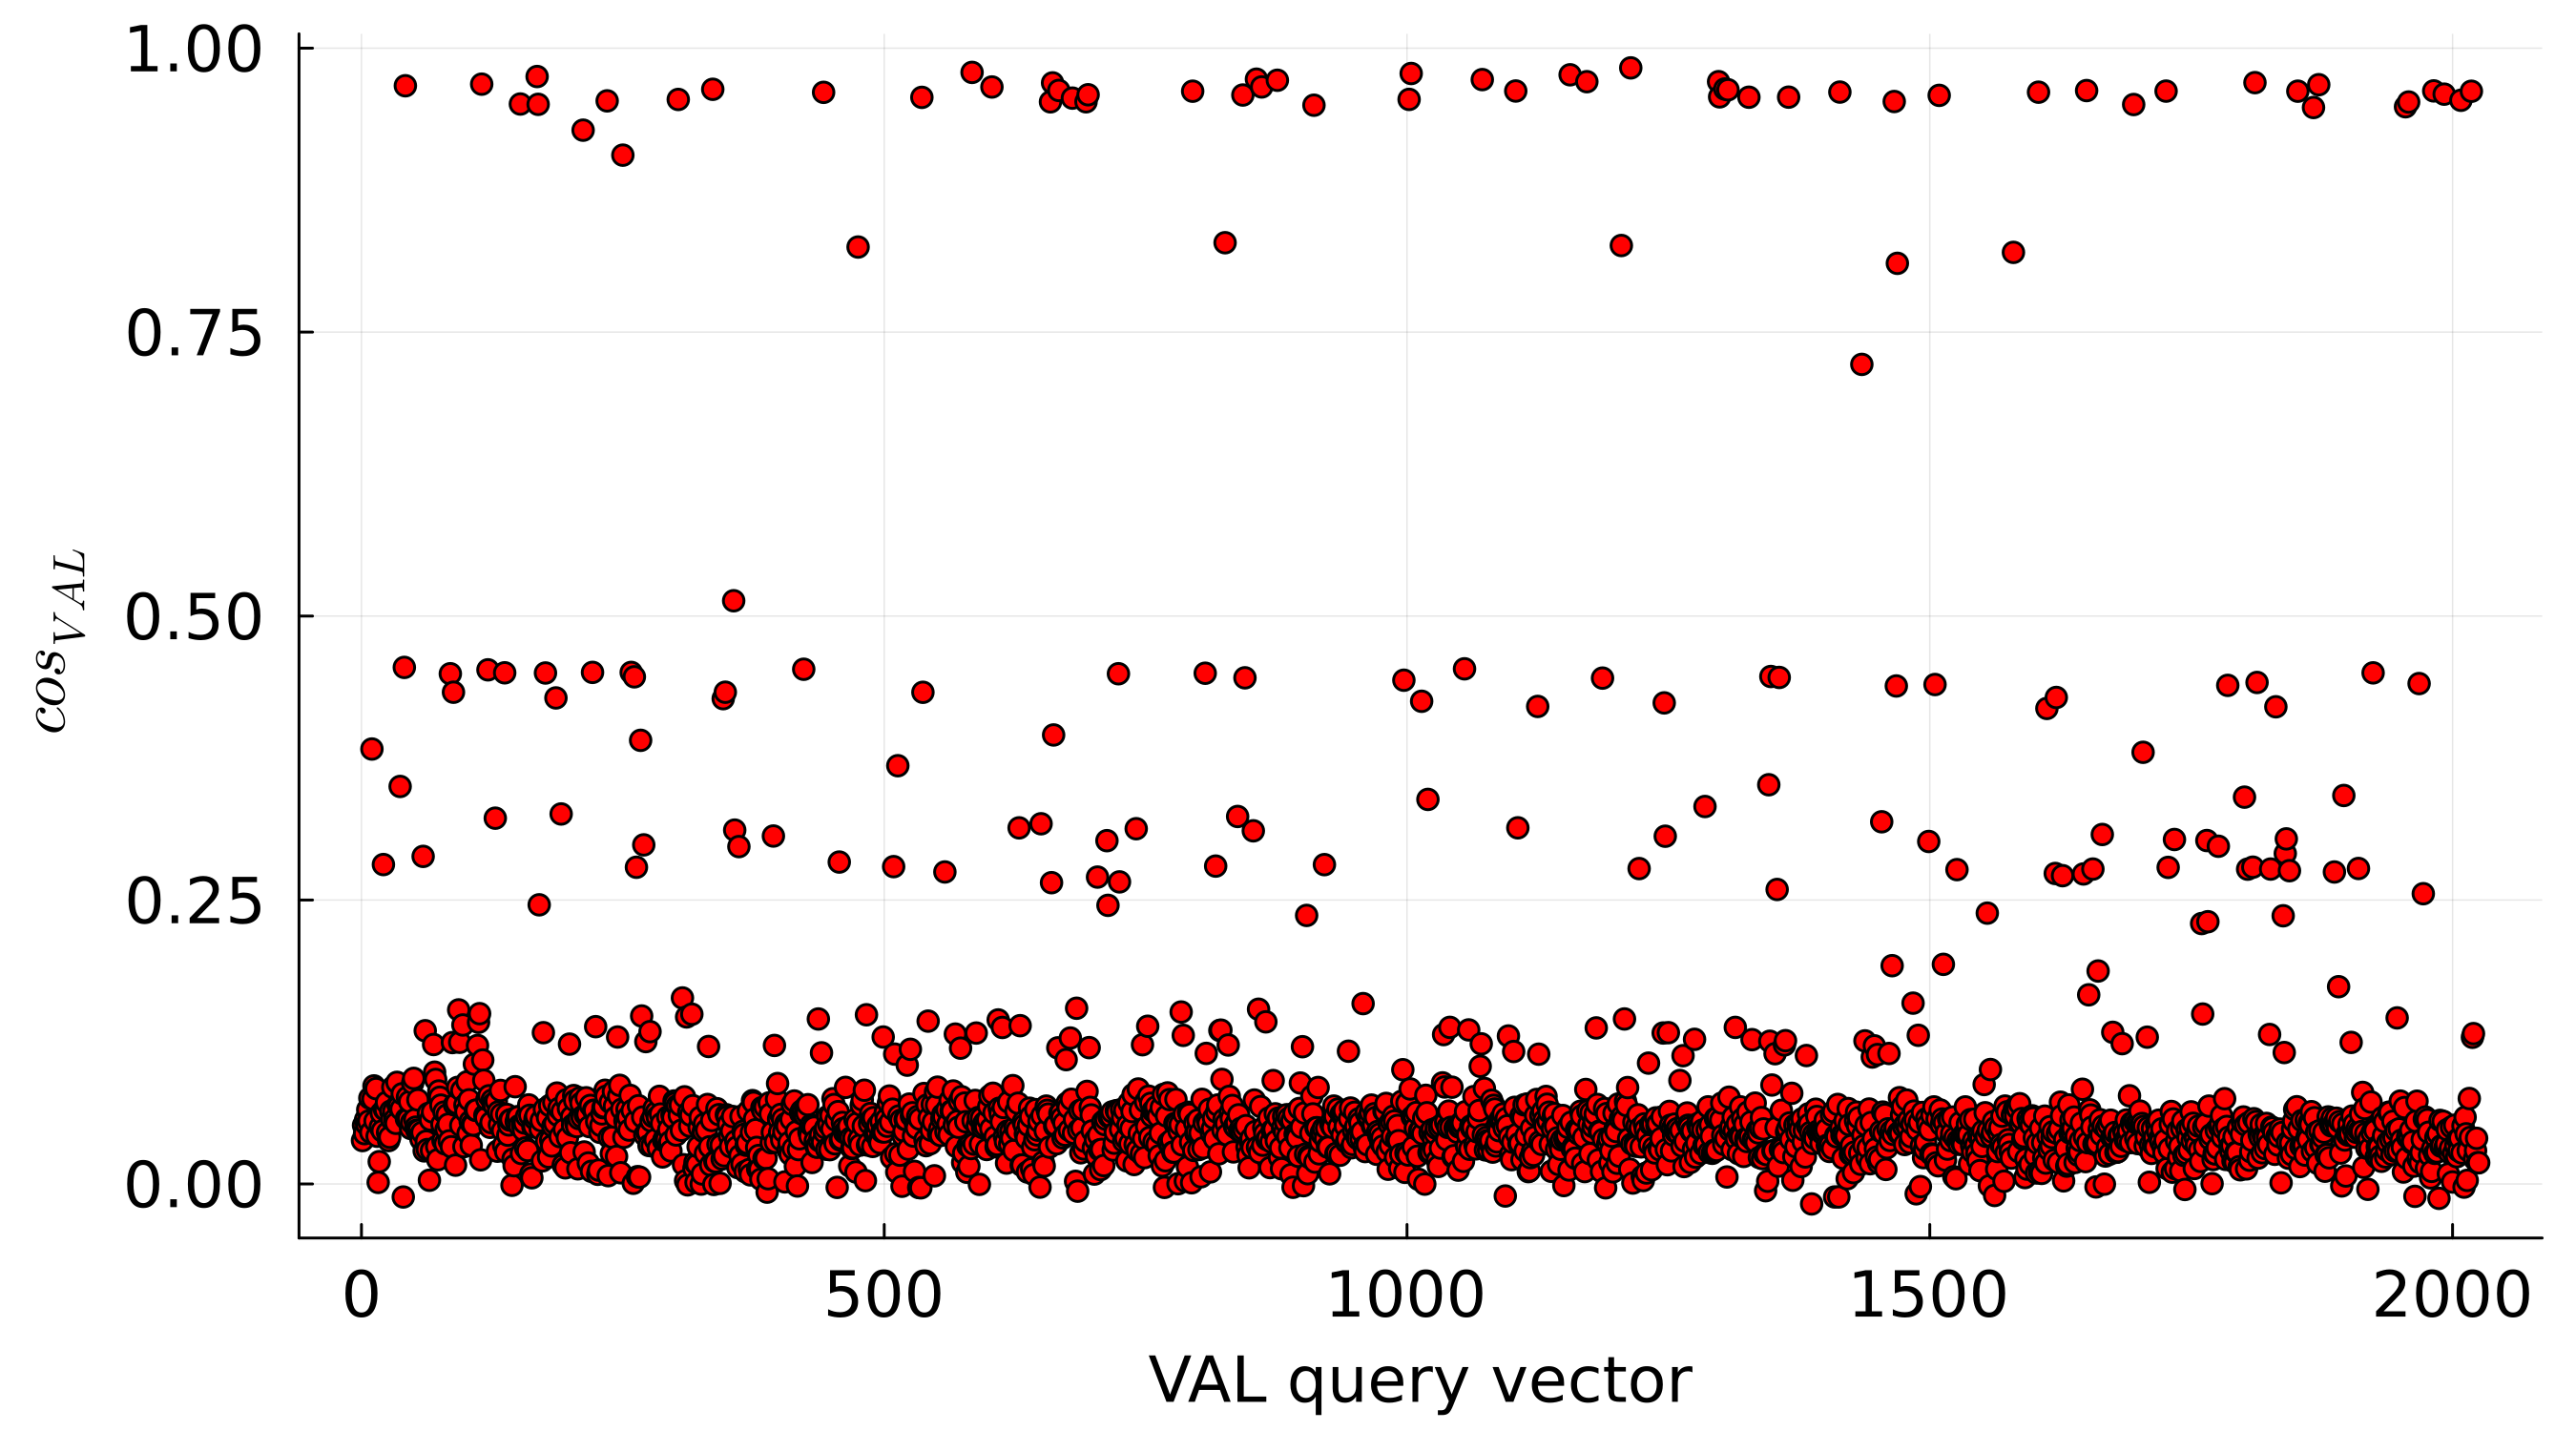
\includegraphics[width=\textwidth]{phalp_cnn_rand_learningV}
        \caption{VALs embedded using using random amino acid vectors \textit{via} the convolutional embedding method}
        \label{fig:subfig-e}
    \end{subfigure}
    \hfill
    \begin{subfigure}{0.48\textwidth}
        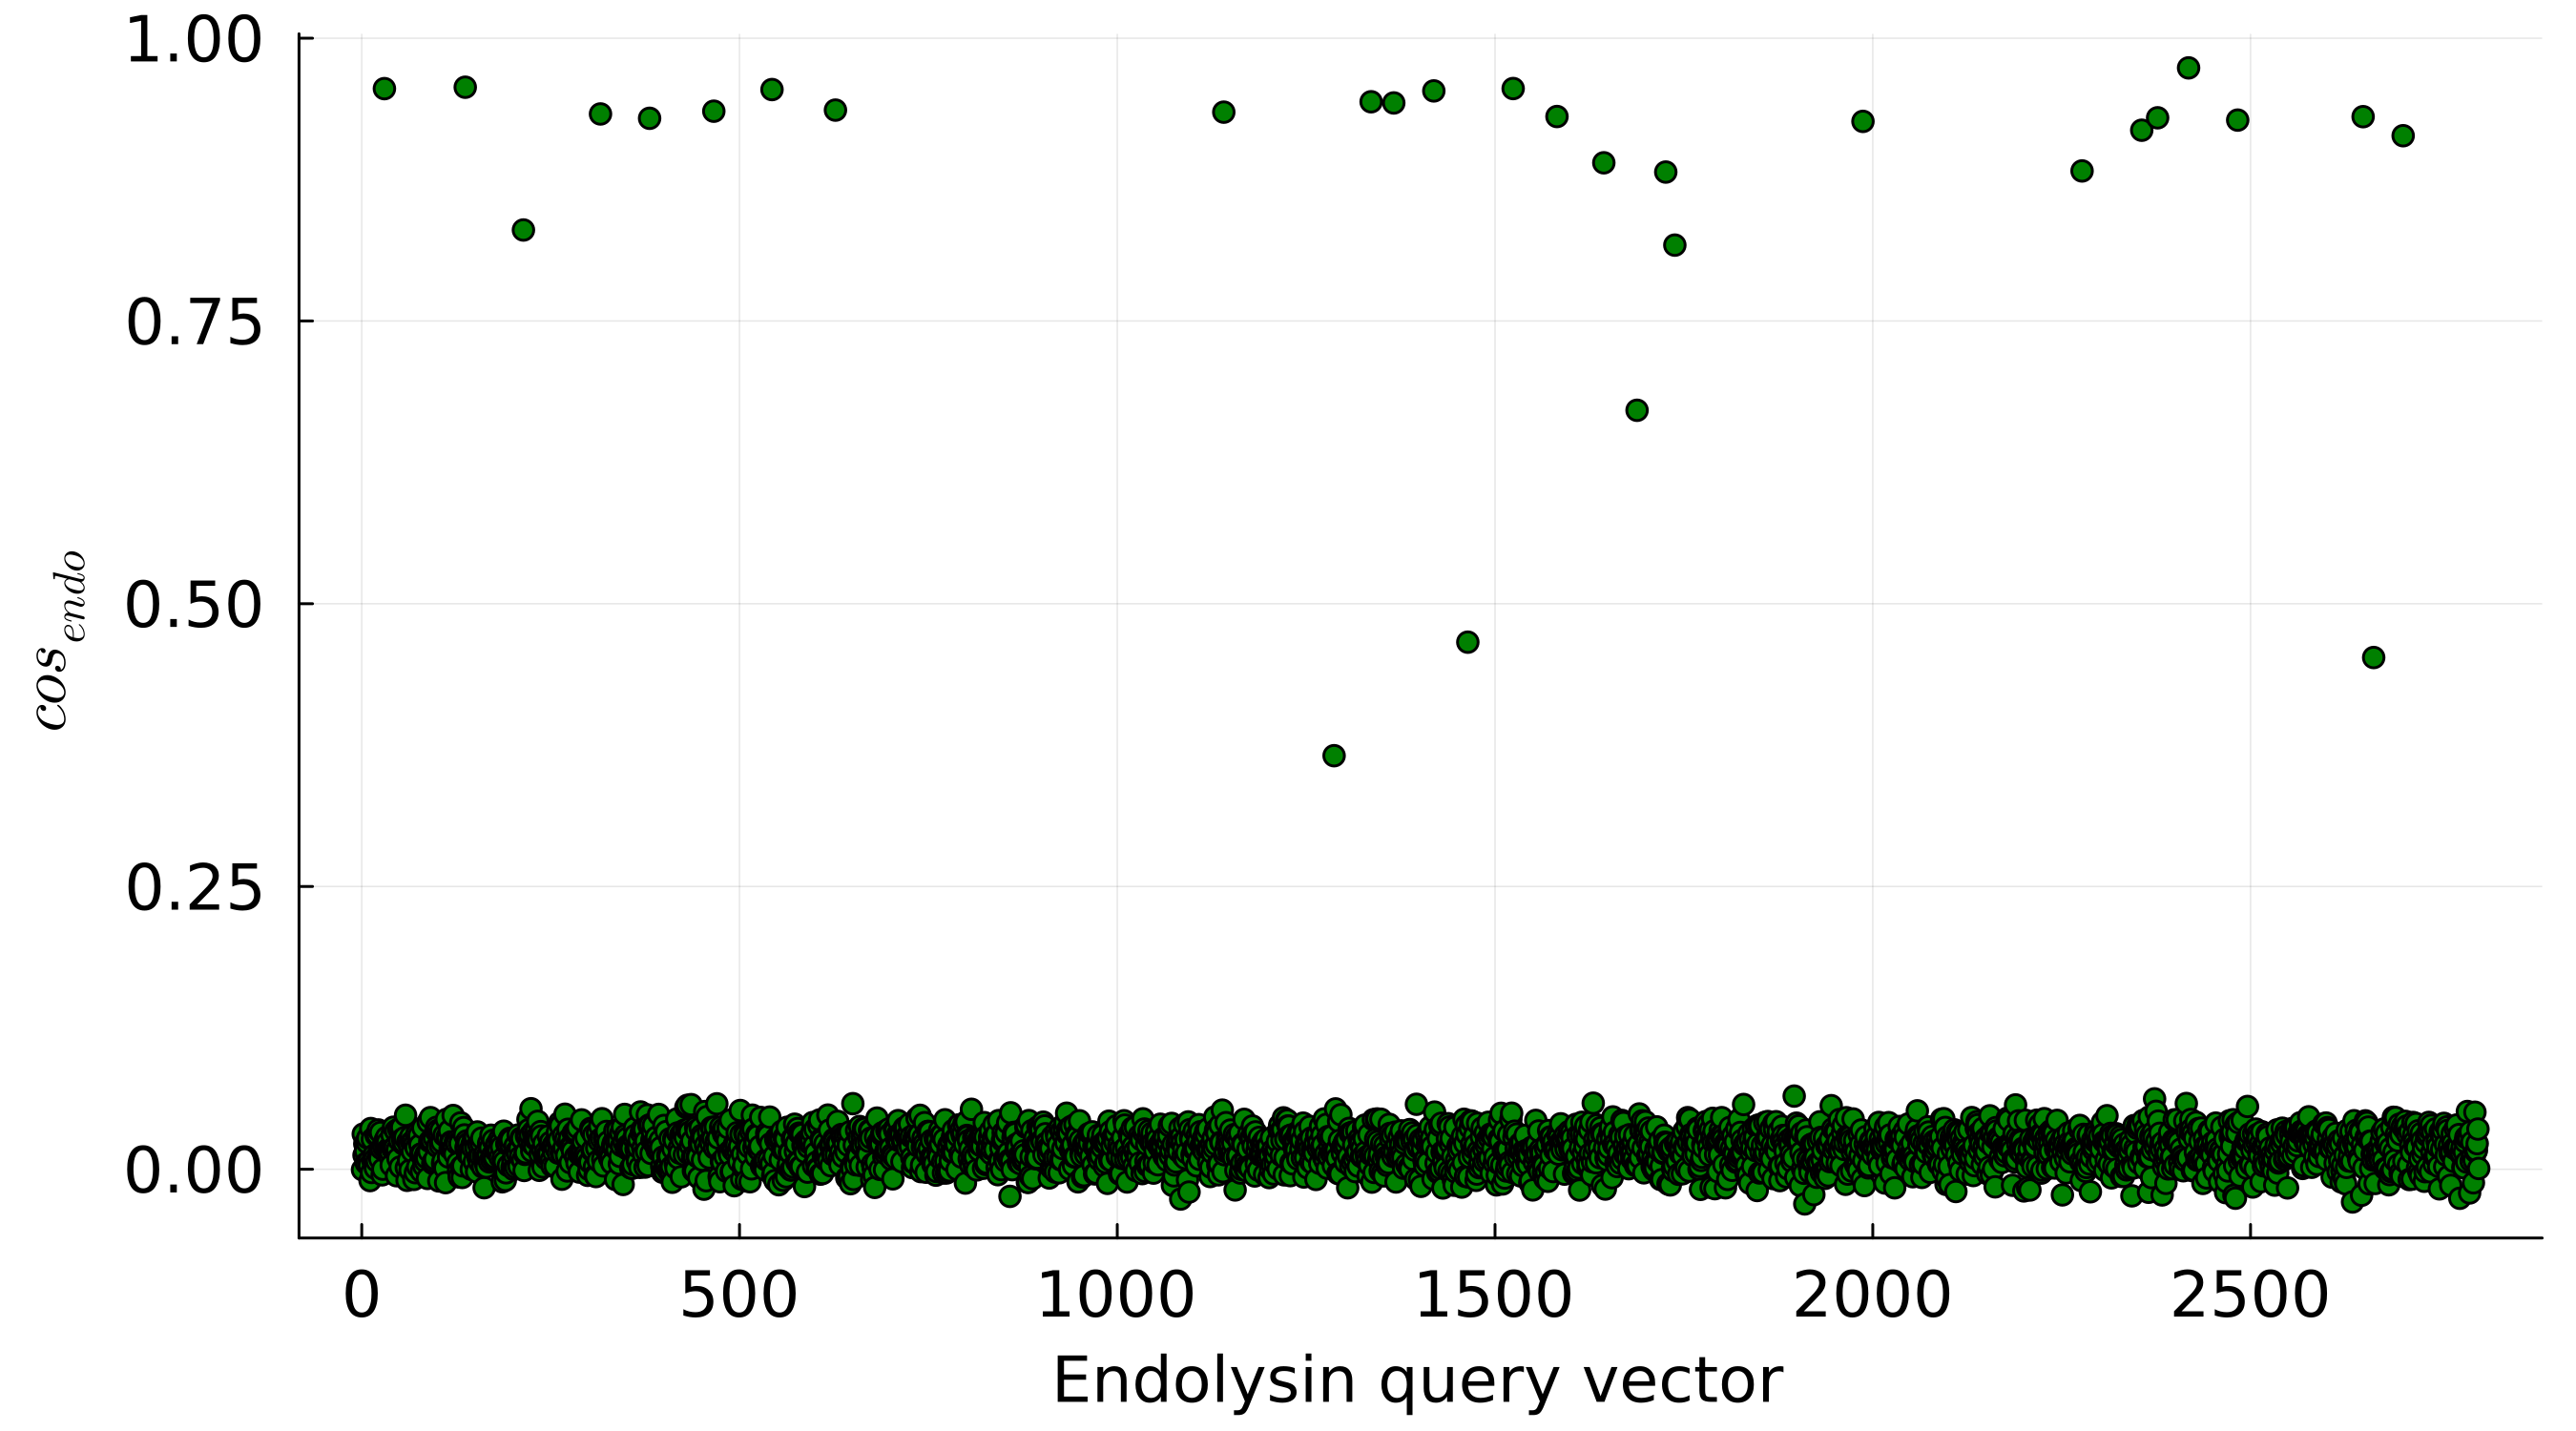
\includegraphics[width=\textwidth]{phalp_cnn_rand_learningE}
        \caption{Endolysins embedded using random amino acid vectors \textit{via} the convolutional embedding method}
        \label{fig:subfig-f}
    \end{subfigure}
    
    \begin{subfigure}{0.48\textwidth}
        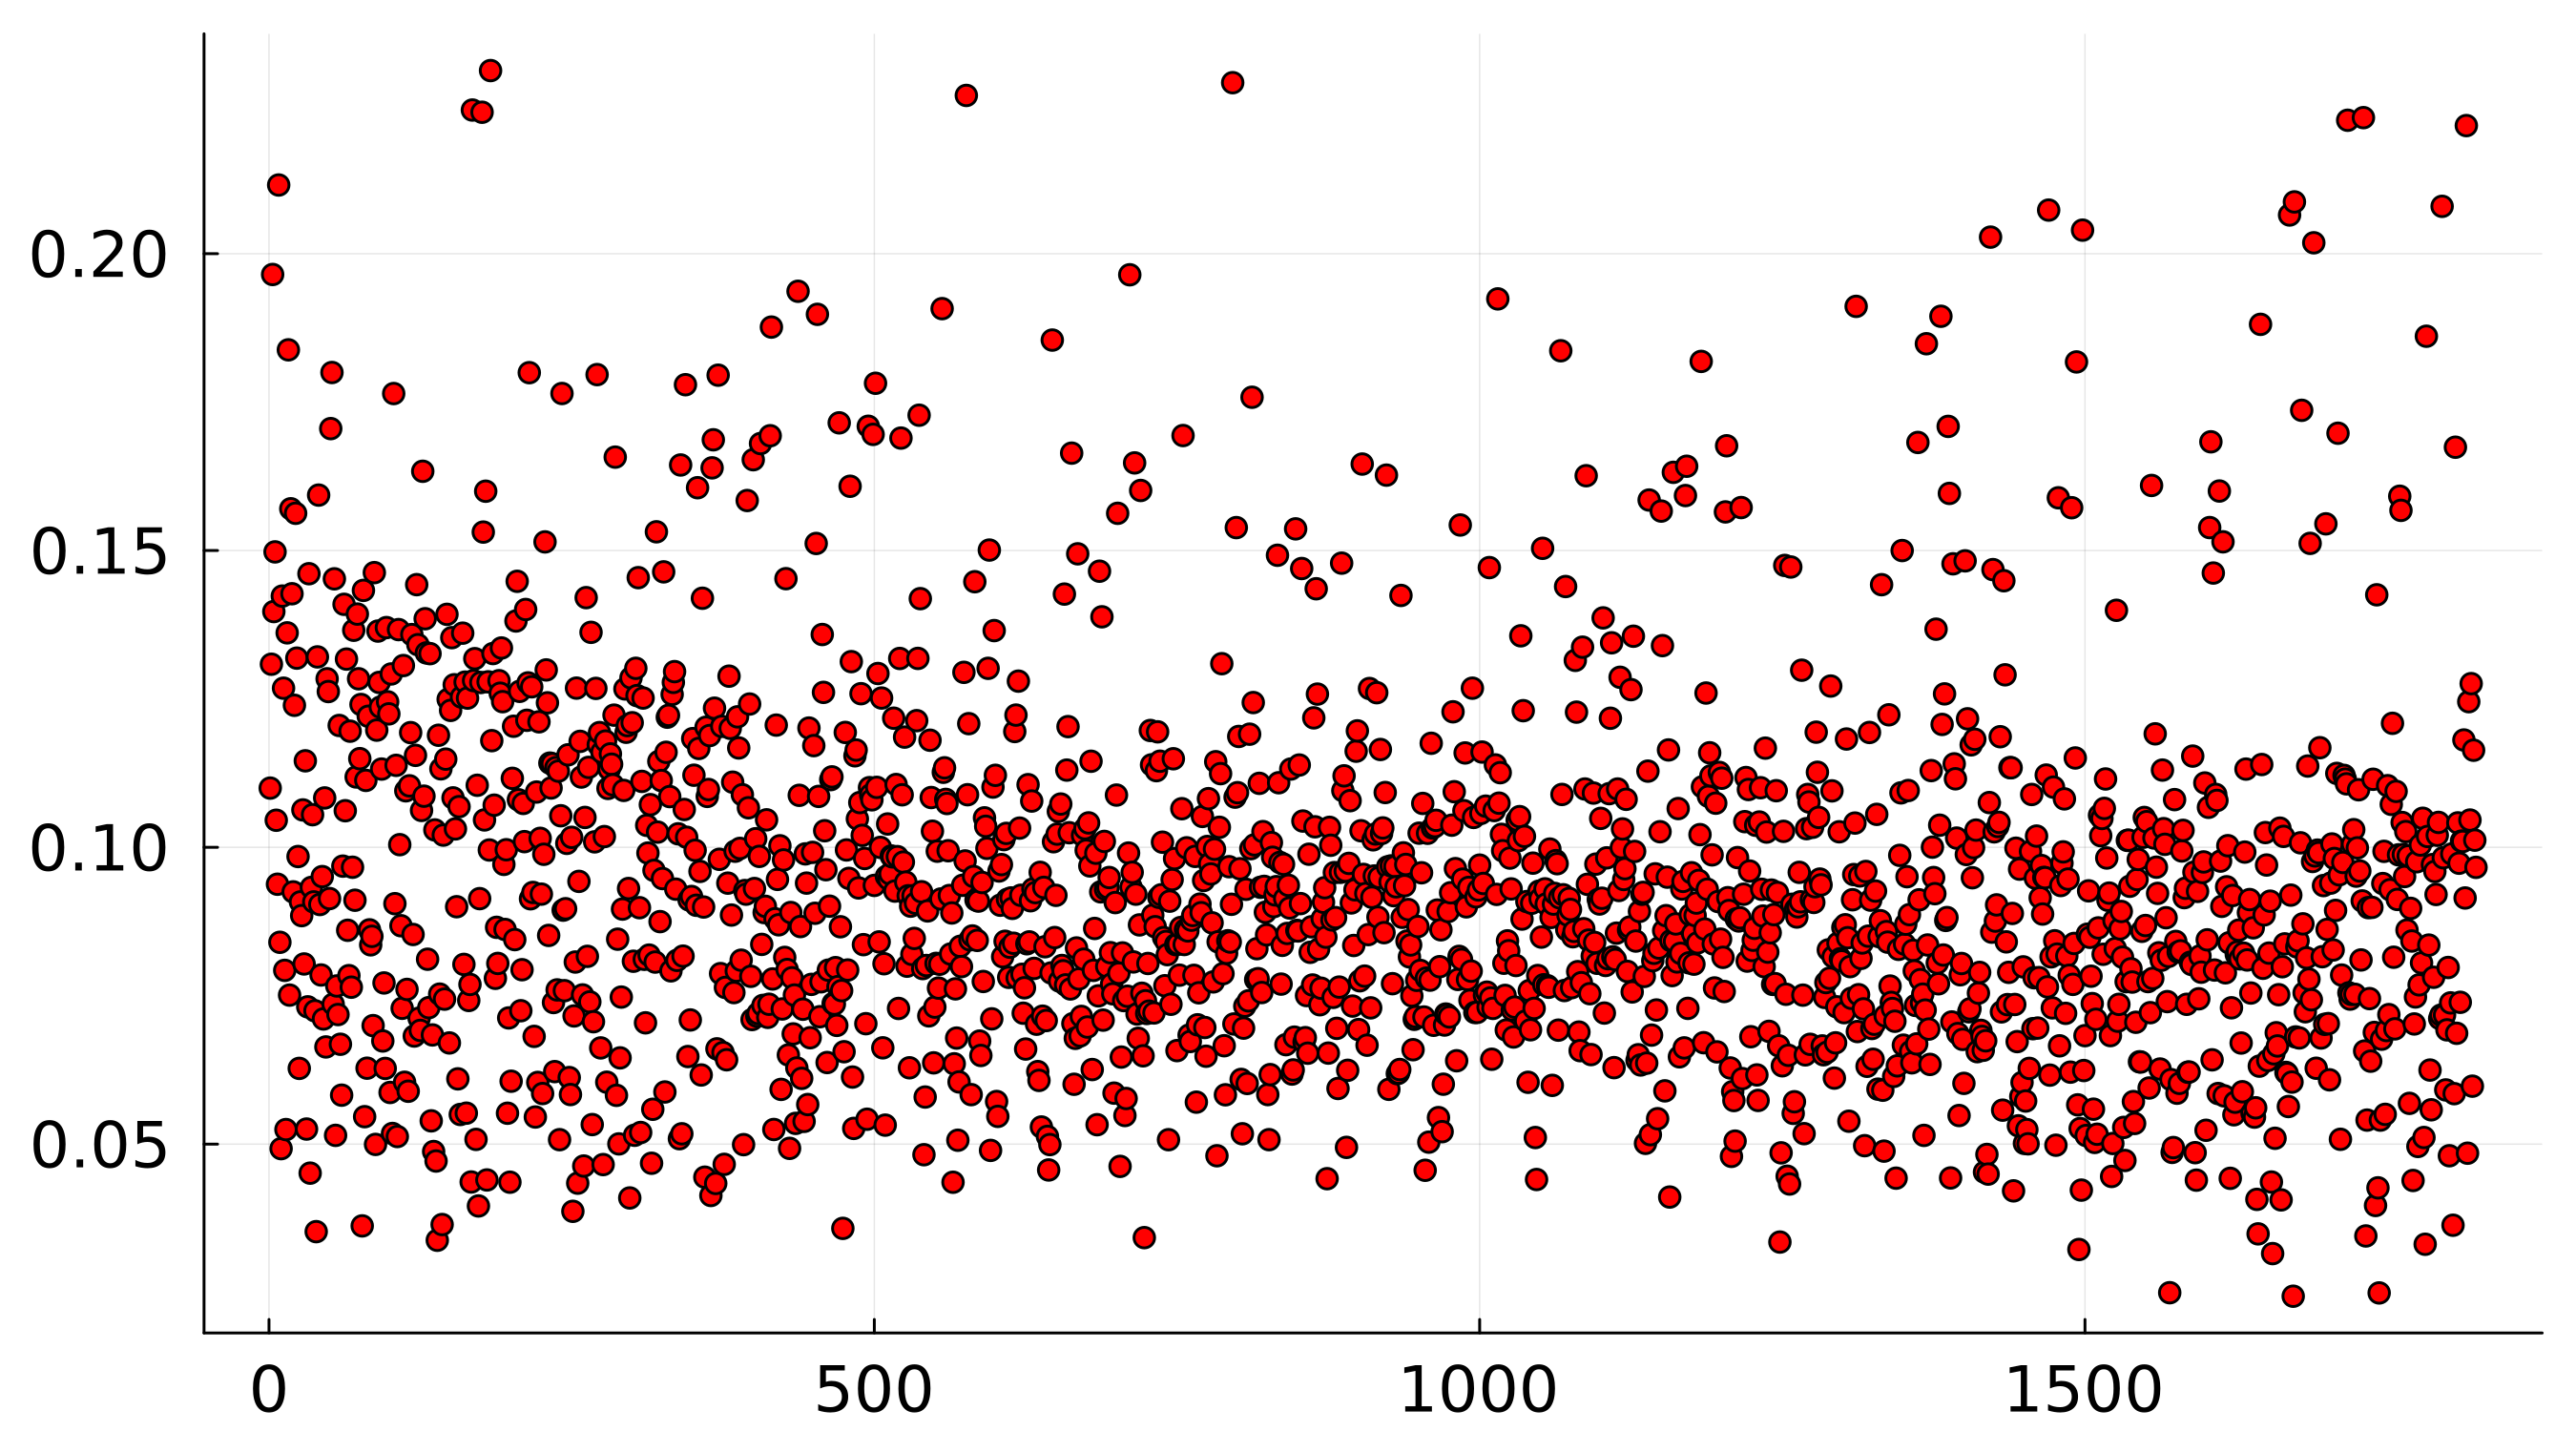
\includegraphics[width=\textwidth]{phalp_cnn_esm_learningV}
        \caption{VALs embedded using projected ESM-2 amino acid vectors \textit{via} the convolutional embedding method}
        \label{fig:subfig-g}
    \end{subfigure}
    \hfill
    \begin{subfigure}{0.48\textwidth}
        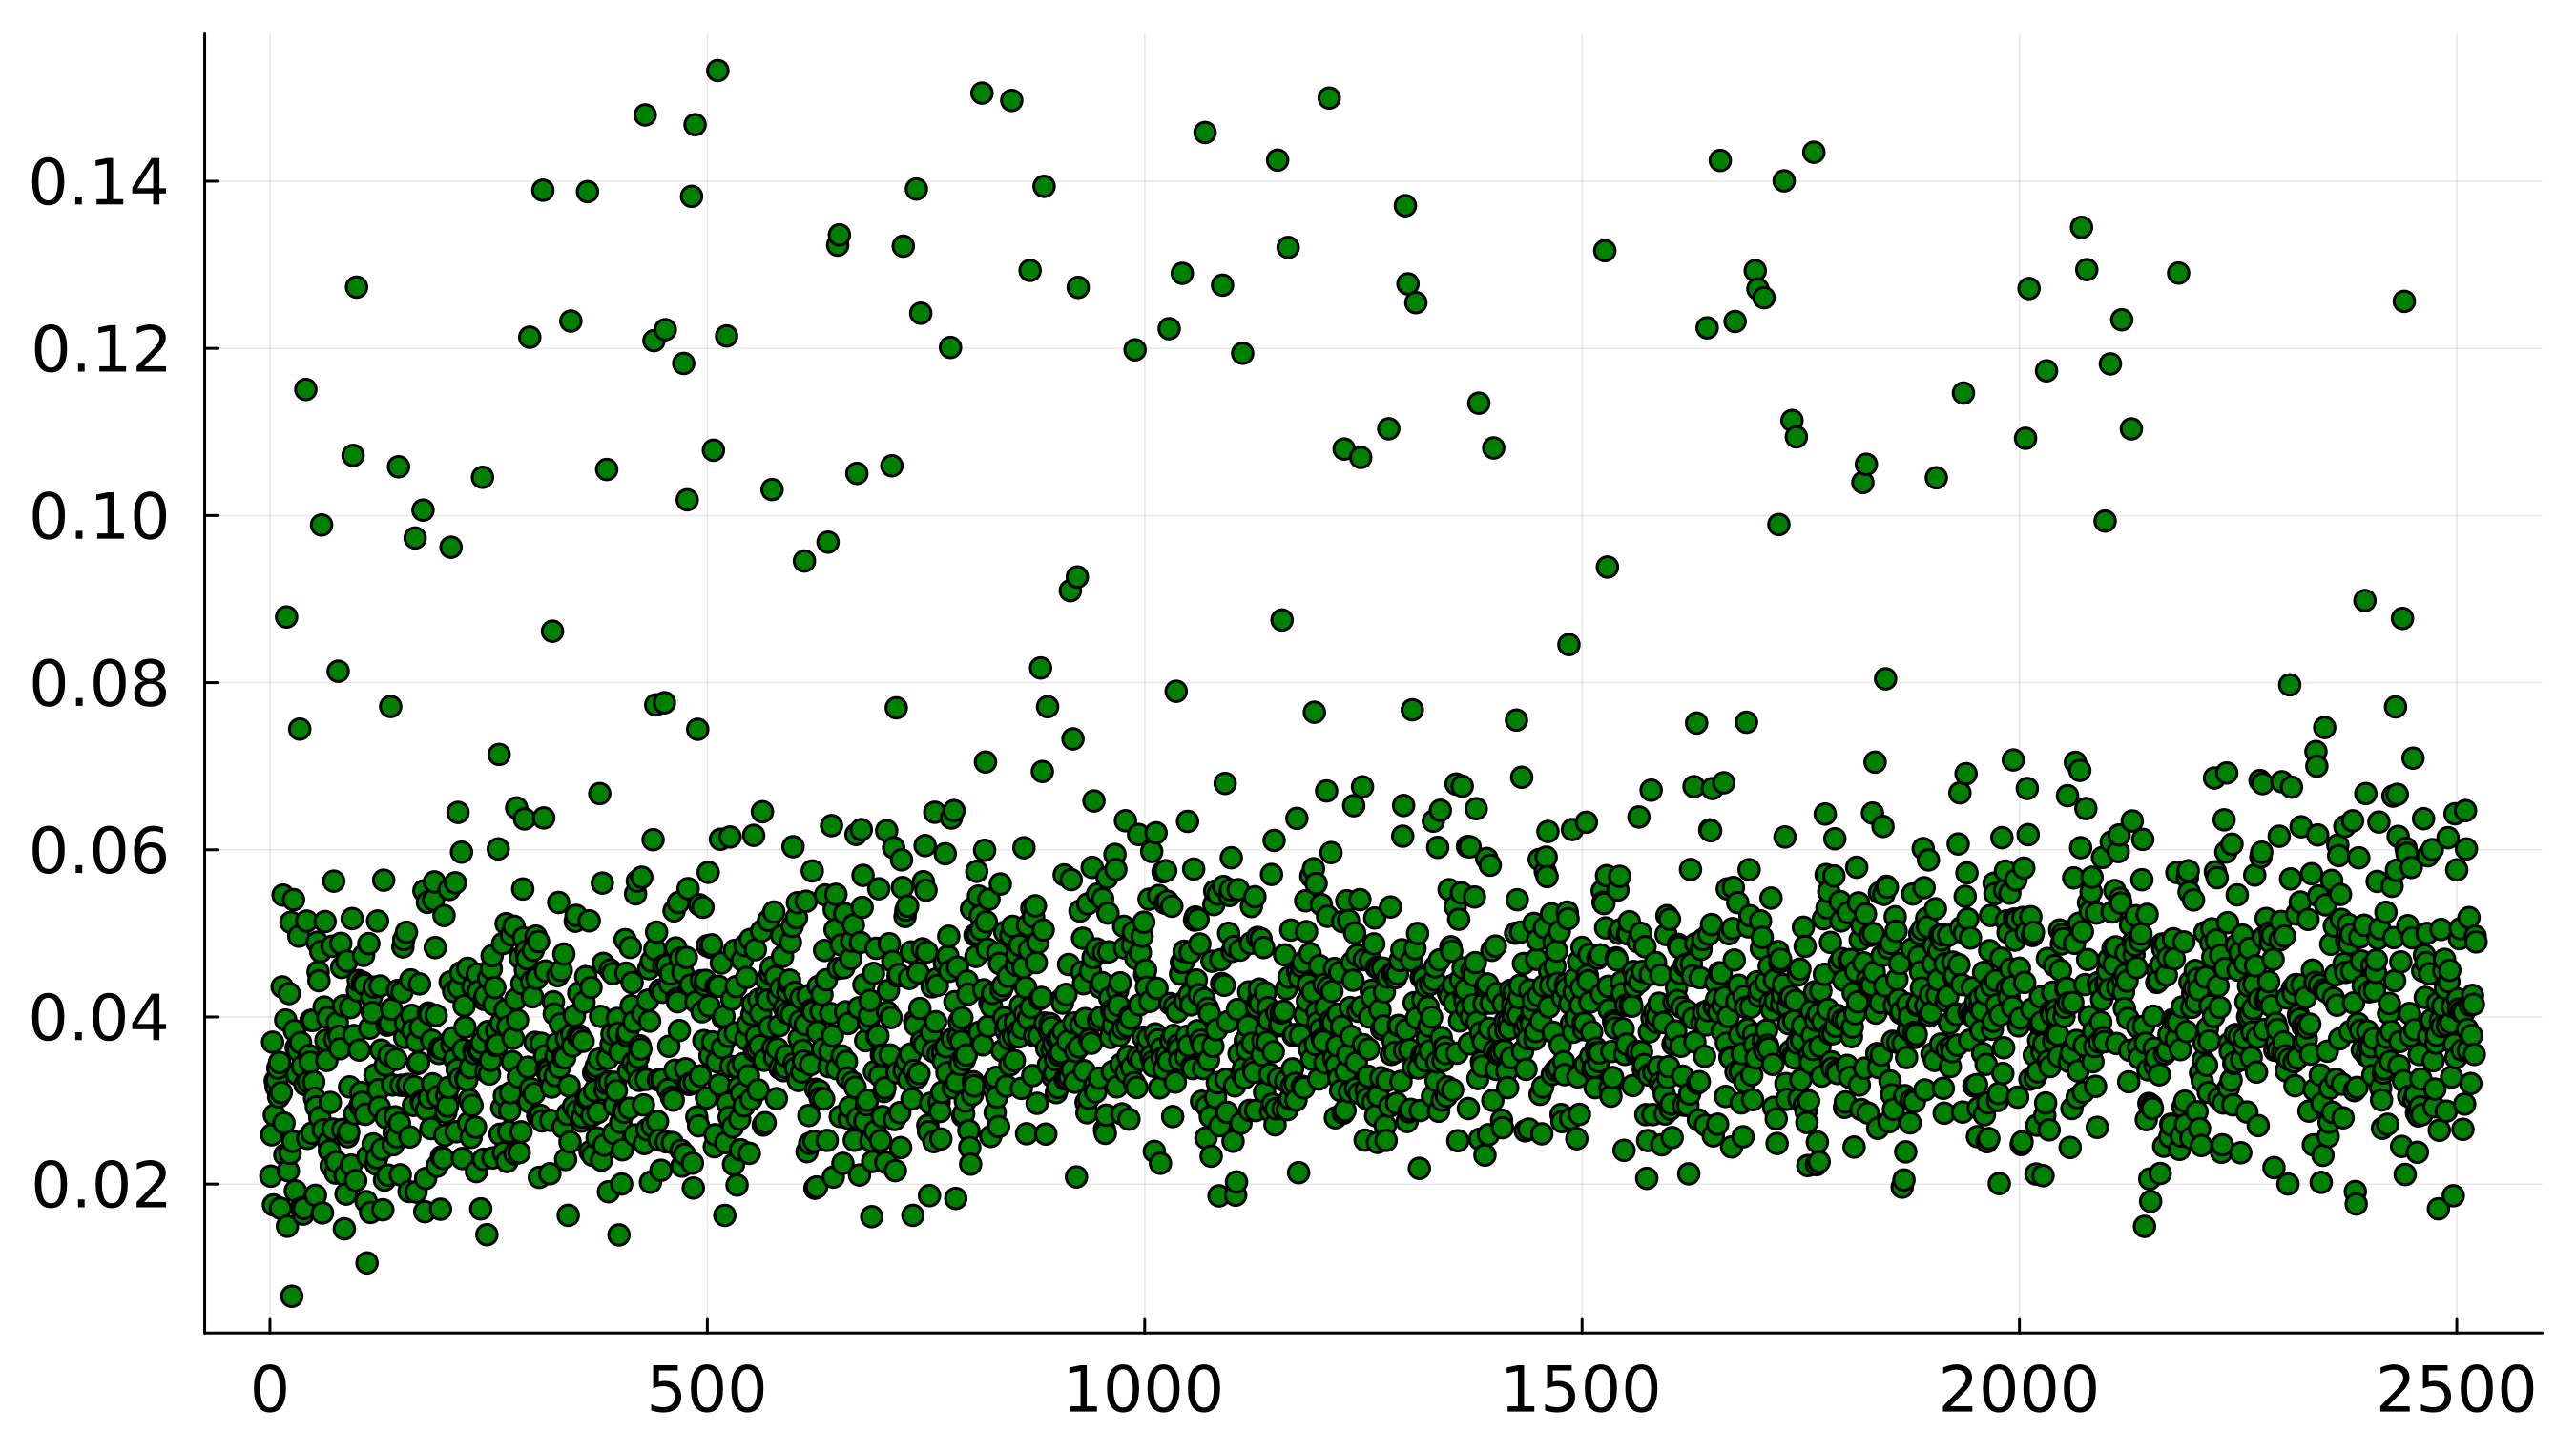
\includegraphics[width=\textwidth]{phalp_cnn_esm_learningE}
        \caption{Endolysins embedded using projected ESM-2 amino acid vectors \textit{via} the convolutional embedding method}
        \label{fig:subfig-h}
    \end{subfigure}
    
    \caption{Cosine similarity between a query vector and the class vector before the weighted update during OnlineHD single-pass training procedure. Trained using hyperdimensional embeddings from all protein sequences in the PhaLP dataset whose types were manually annotated, red representing VALs and green representing endolysins.}
    \label{fig:main}
\end{figure}

Another approach to monitor the training procedure is to track the two class vectors $C_{VAL}$ and $C_{endo}$ individually. For each query vector with a known label $l$, we calculate the cosine similarity $cos(V_{l}, C_{l})$. This method allows us to observe the model's adaptation and refinement of its internal representation of the two classes before it predicts a query vector during the training process. The distance between a query vector and a class vector is proportional to the update weight, so we expect the cosine similarities to generally increase as the model learns. The results are shown in Figure~\ref{fig:main}.

In this case, the VAL vector shows near-consistent weight updates, indicating a high likelihood of the dataset being diverse as the cosine similarities don't seem to decrease. This consistent learning pattern also suggests that the method effectively extracts and learns from the diverse information embedded in the dataset. In general, we see a higher variation in cosine similarities for VAL vectors, which suggests that virion-associated lysins are more diverse in sequence compared to endolysins. This also confirms our earlier findings. We also notice higher overall similarities between the query vectors and the VAL vector when using the BoW-method with projected ESM-2 vectors compared to other embedding methods, which aligns with this model's superior performance. The endolysin vector appears to be updated at a constant rate too, with less variation in similarities. As observed with the VAL vectors, the similarities between the query vectors and the endolysin vector are higher when the embeddings are created using the BoW-method with projected ESM-2 vectors.

\begin{figure}[ht!]
    \centering
    \begin{subfigure}{0.48\textwidth}
        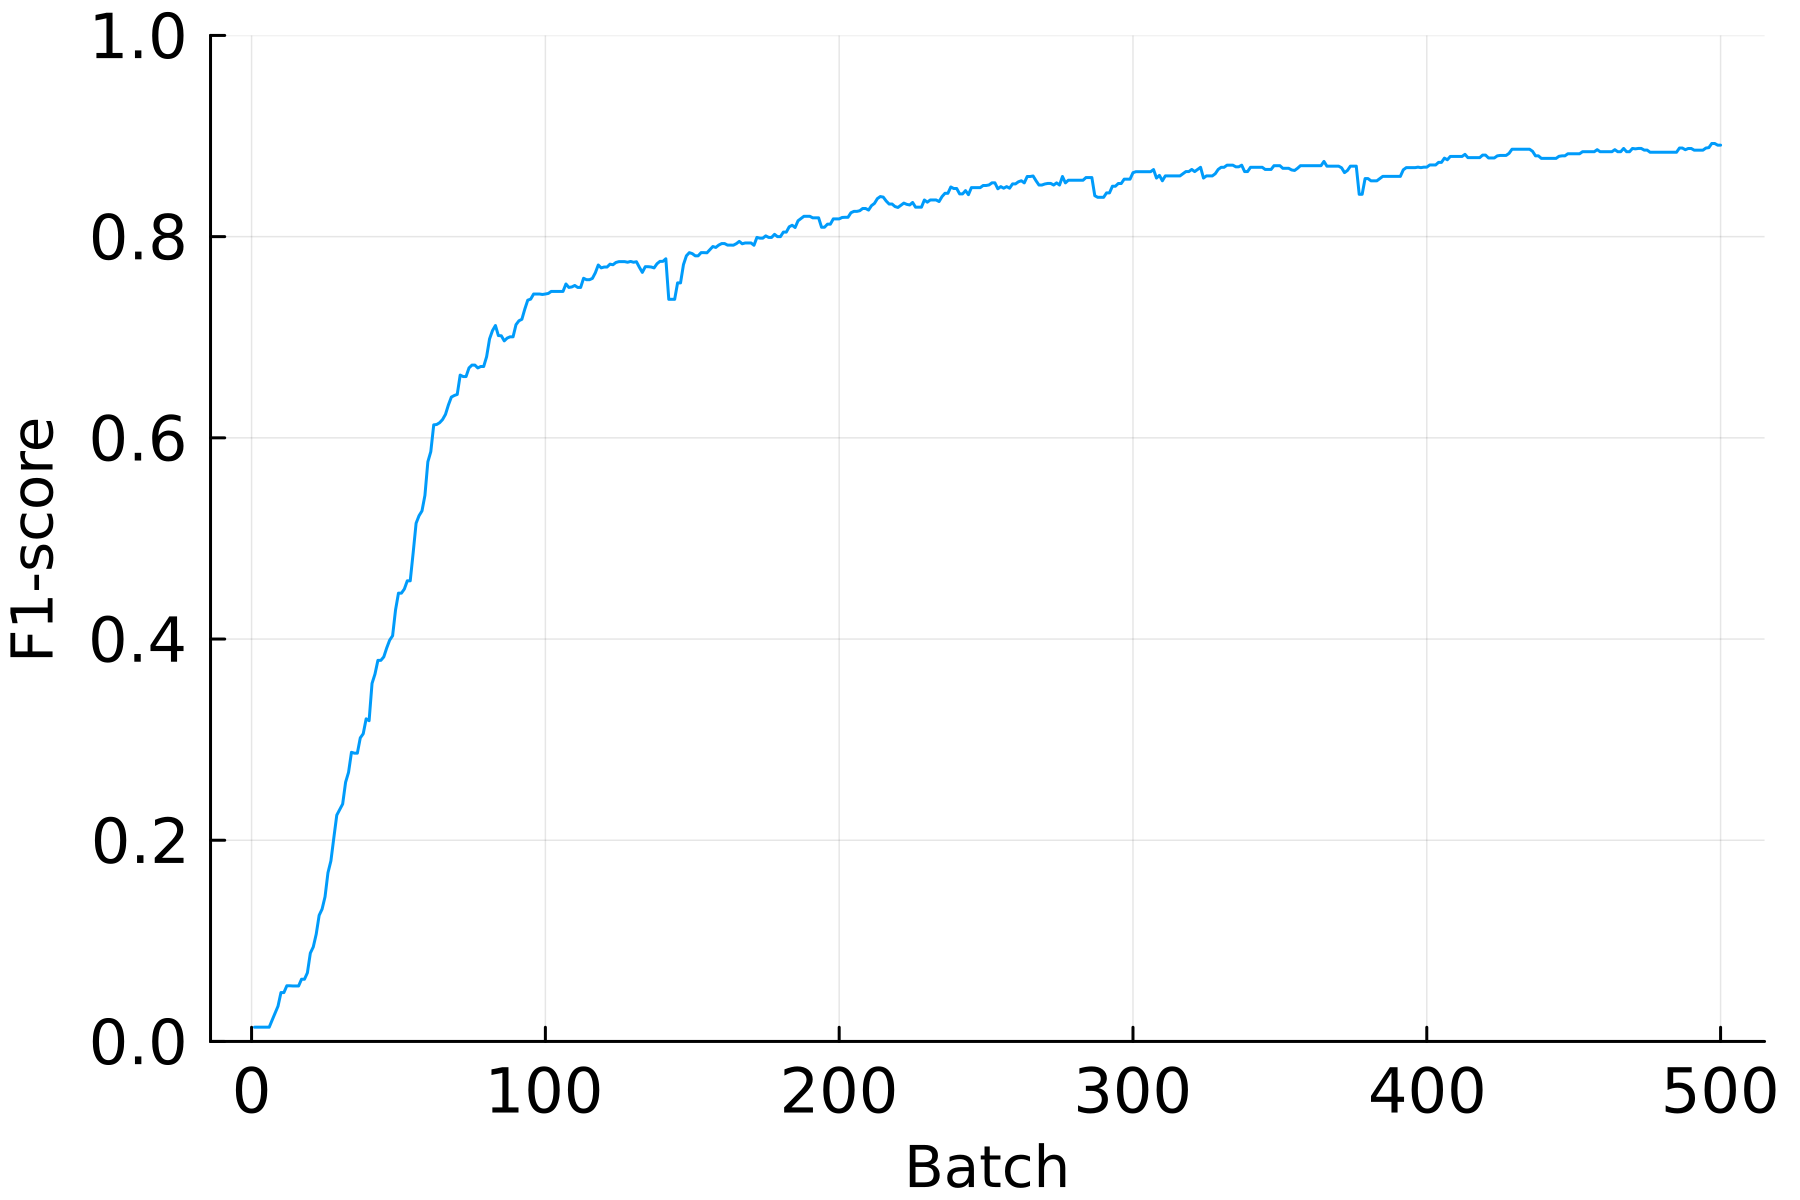
\includegraphics[width=\textwidth]{phalp_bow_rand_score}
        \caption{Embeddings using random amino acid vectors, made \textit{via} the bag-of-words embedding method}
        \label{fig:subfig-a3}
    \end{subfigure}
    \hfill
    \begin{subfigure}{0.48\textwidth}
        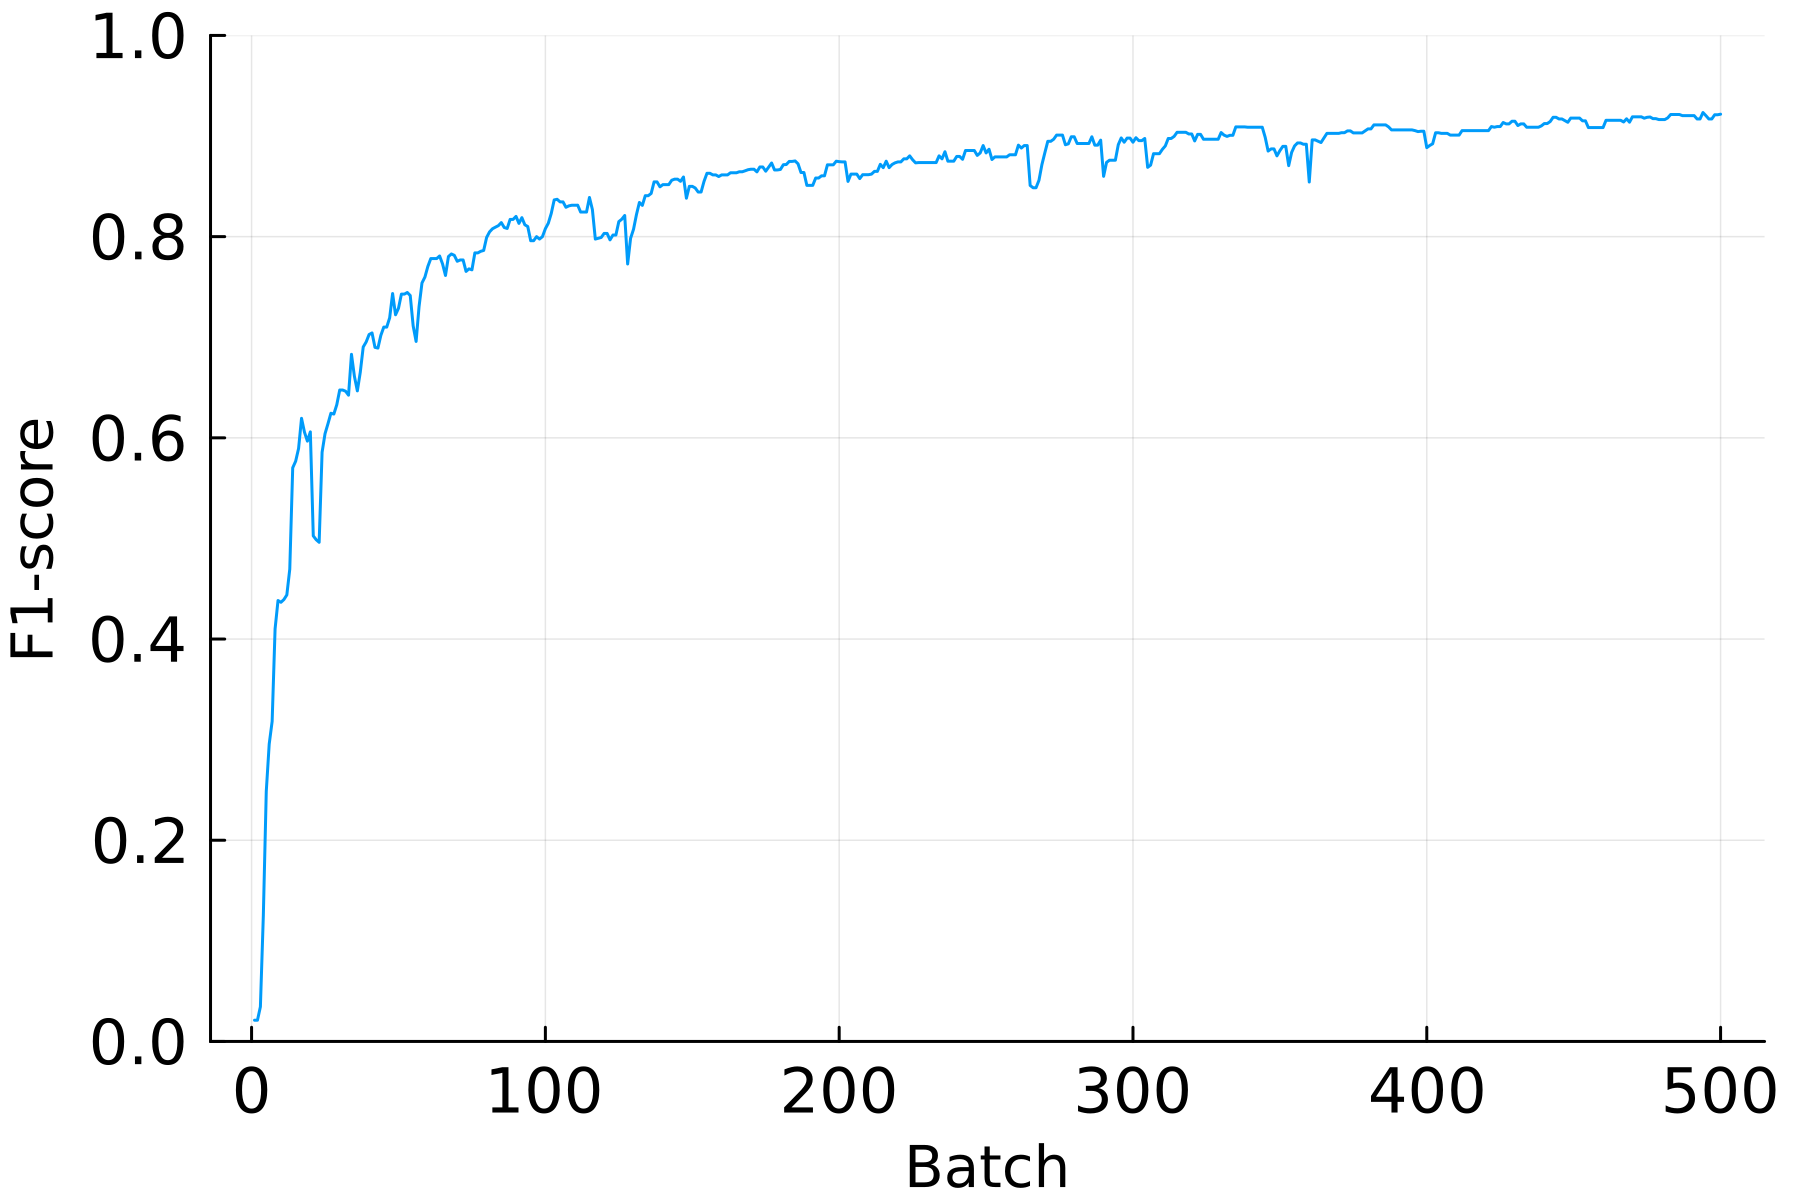
\includegraphics[width=\textwidth]{phalp_bow_esm_score}
        \caption{Embeddings using projected ESM-2 amino acid vectors, made \textit{via} the bag-of-words embedding method}
        \label{fig:subfig-b3}
    \end{subfigure}
    
    \begin{subfigure}{0.48\textwidth}
        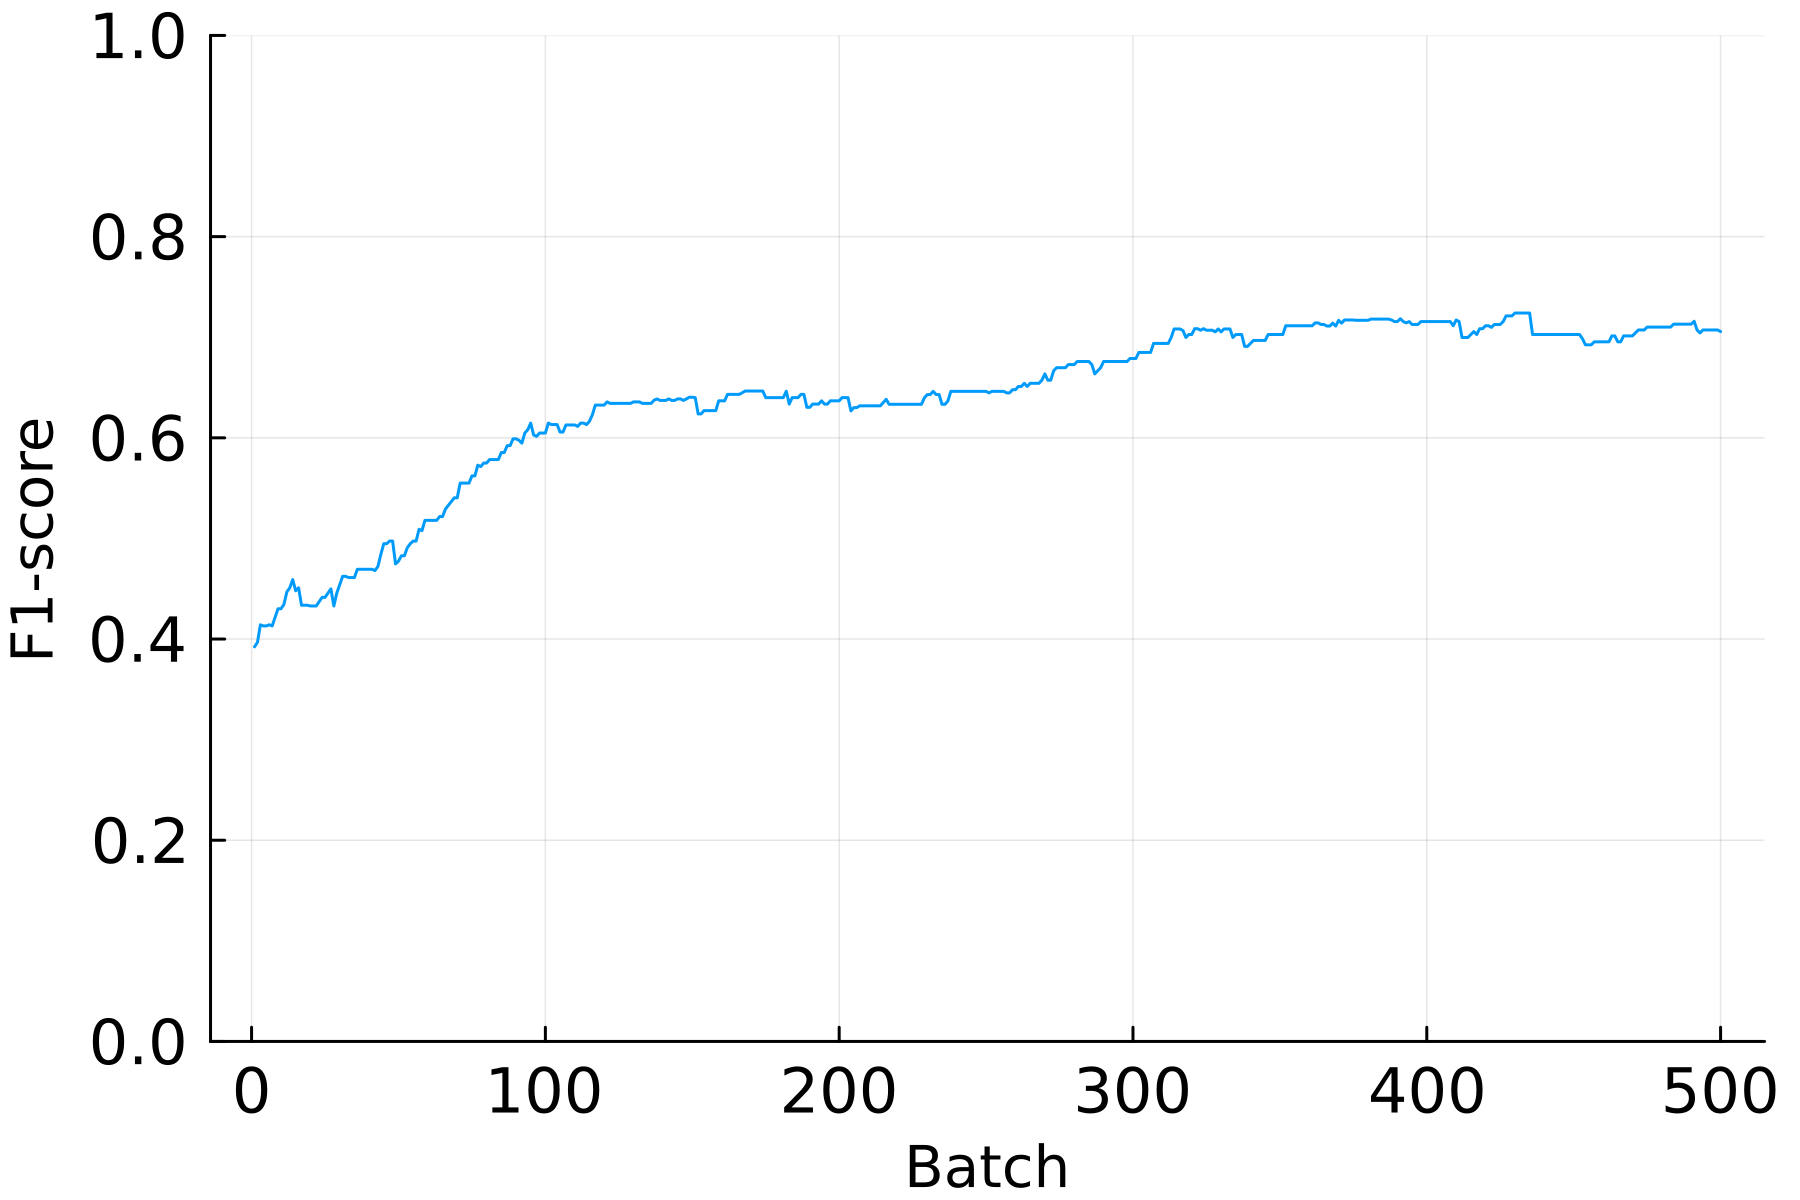
\includegraphics[width=\textwidth]{phalp_cnn_rand_score}
        \caption{Embeddings using random amino acid vectors, made \textit{via} the convolutional embedding method}
        \label{fig:subfig-c3}
    \end{subfigure}
    \hfill
    \begin{subfigure}{0.48\textwidth}
        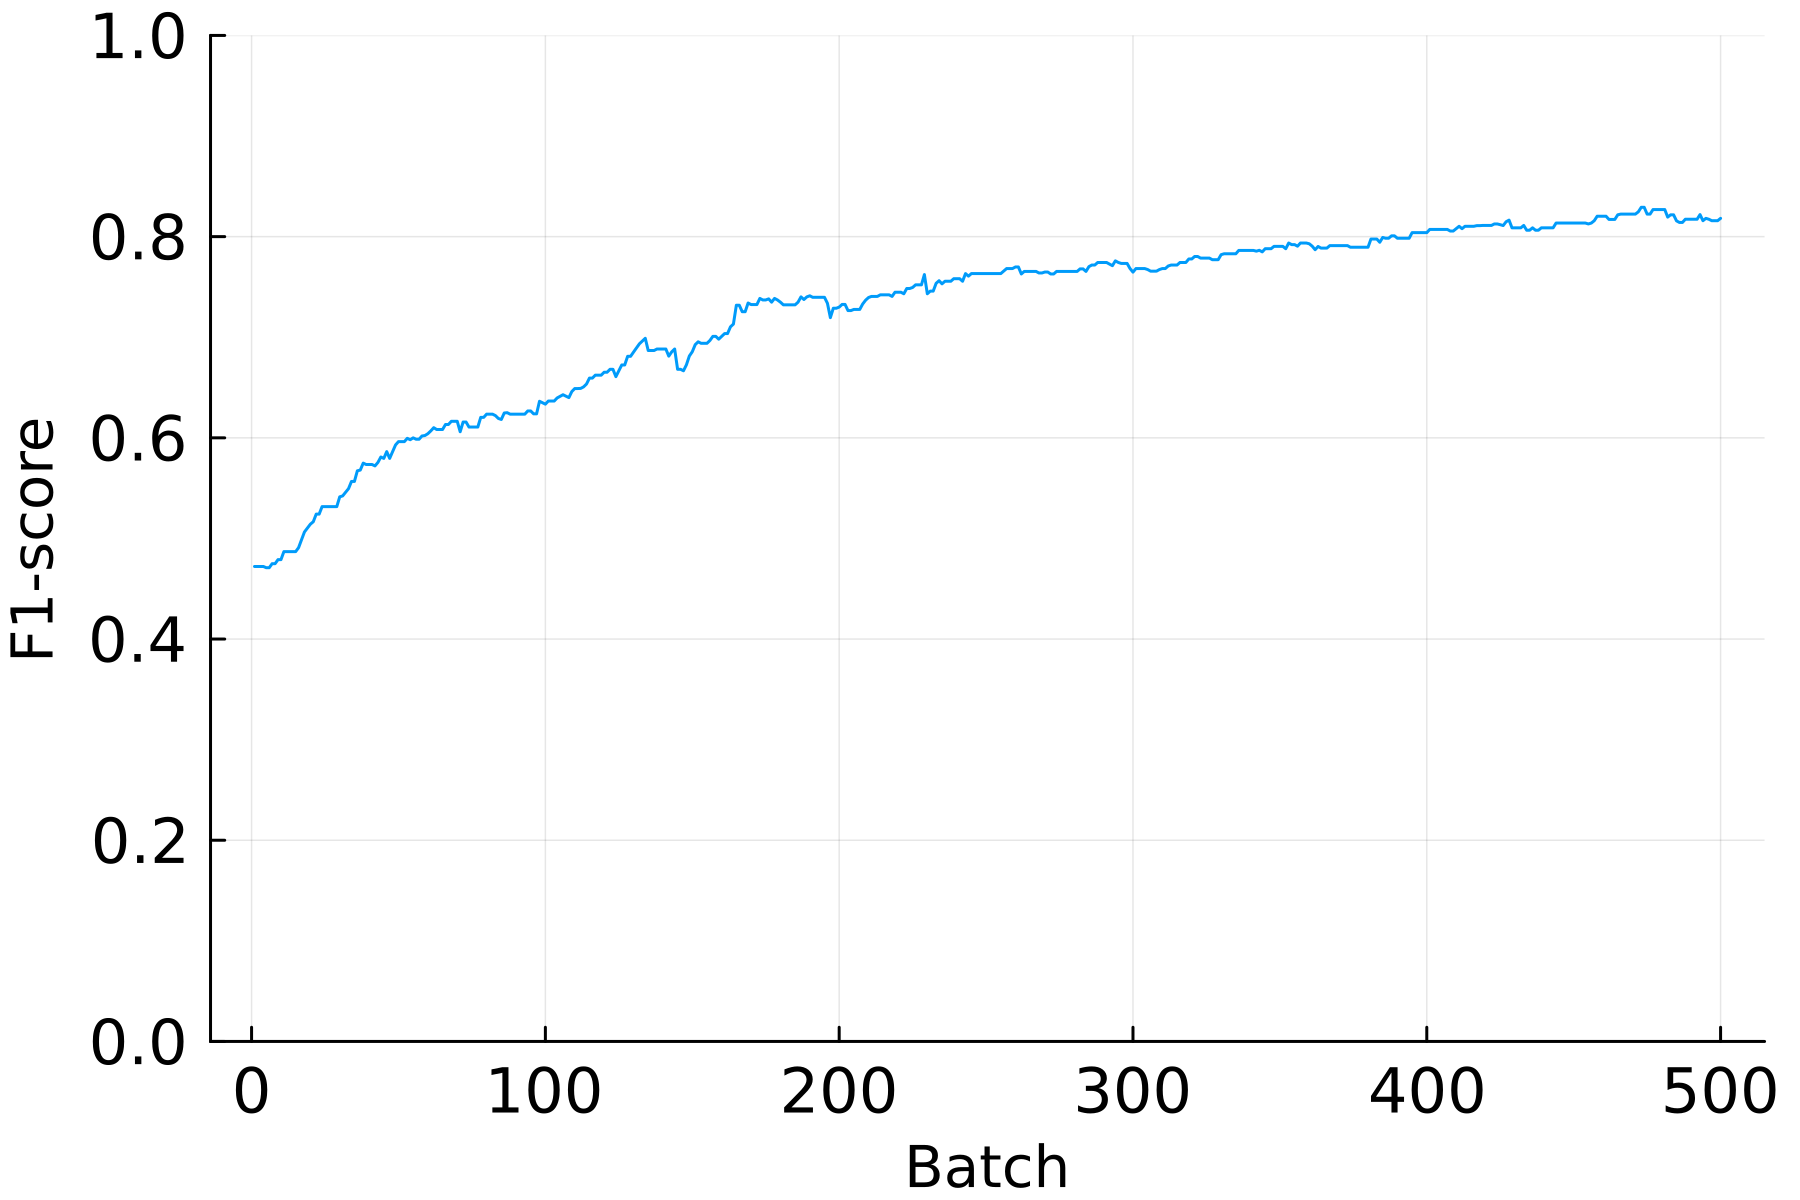
\includegraphics[width=\textwidth]{phalp_cnn_esm_score}
        \caption{Embeddings using projected ESM-2 acid vectors, made \textit{via} the convolutional embedding method}
        \label{fig:subfig-d3}
    \end{subfigure}
    \caption{The F1-score of the OnlineHD single-pass model with a validation set throughout its training procedure. Trained in batches using several kinds of hyperdimensional embeddings from all protein sequences in the PhaLP dataset whose types were manually annotated.}
    \label{fig:main39}
\end{figure}

Instead of looking at the inner workings of the OnlineHD method, the training progress of an OnlineHD model in terms of performance has been monitored. This progress is visualized in Figure~\ref{fig:main39}. Upon initial observation, it is apparent that the models trained with embeddings generated using the convolutional method exhibit superior performance from the outset. This higher starting point might be partially attributed to the random initialization of the model. However, a common characteristic observed across all models is that their performance tends to stagnate after roughly 100 batches, which corresponds to roughly 870 sequences in our case. This observation suggests that hyperdimensional computing-based classification methods may exhibit promising performance and effectively capture essential information, even after being exposed to just a small fraction of the training data, which is an intriguing finding for further exploration.

\section{Discussion}
The low scores of the naive additive methods are likely due to the possibility of oversaturation of the class vectors as discussed in section~\ref{sec:dis3}. Thus, using the rudimentary model works only for very small datasets, as seen in the examples in chapter~\ref{sec:example}. The ability of this method to learn from a small dataset can be very useful, but backfires in terms of performance when applied to large and diverse datasets as we have seen in the case of classifying protein sequences from the PhaLP database.

This issue is mitigated in the OnlineHD method when used in classifications as it applies weights to class vector updates. This results in a substantial increase in performance. When paired with an iterative retraining procedure its performance comes close to the performance of established machine learning methods paired with binary hyperdimensional sequence embeddings. The OnlineHD methods require real-valued vectors, but still show much higher computational efficiencies compared to established machine learning methods.

From the results in Figures~\ref{fig:main2} and ~\ref{fig:main}, we could not conclude using similarities of query vectors to the class vectors as a metric for training monitoring, as these more likely represent the variety in the training data, especially visible in Figure~\ref{fig:main} as the better-performing models show that they capture more of the intricacies of the input data.

Looking at OnlineHD's performance during its training procedure in Figure~\ref{fig:main39}, we noticed that it is able to capture a lot of information with only a small set of the data, which warrants further study. To further investigate the potential of OnlineHD for protein-level classification in future research, we could investigate how it could classify the sequences based on other types of information present in the PhaLP database such as host type and domains.

Upon comparing various methods for amino acid encoding, we find that dimension-reduction methods tend to capture more information from sequence embeddings created with projected ESM-2 vectors. This observation is consistent with our other finding where we consistently noted an enhanced performance in our classification task using these amino acid vectors. However, our analysis was limited to a single dataset and one specific task; consequently, further investigation is essential. Future studies should focus on the development and evaluation of alternative tasks, while also testing the applicability of this method across various biological datasets.

As for the sequence embedding methods, while no visual differences were discernible after applying PCA to the protein sequences, the results varied subtly depending on the specific model used for classification. Therefore, it appears that there may not be a significant difference in how information is being captured between the two sequence embedding methods in our case. This may indicate that encoding positional information into the k-mers may not be necessary to capture information on protein sequences as the BoW-method captures enough essential information in our case. Nevertheless, future research should discern the potential utility of this in the context of other datasets and predictive tasks.